\documentclass[a4paper,11pt]{article}
\usepackage[T1]{fontenc}
\usepackage[utf8]{inputenc}
\usepackage{lmodern} 
\usepackage[portuguese]{babel}
\usepackage{graphicx}			%para imagens
\usepackage{epstopdf} 			%resolve problemas eps-pdf
\usepackage{fancyhdr}			% para o cabeçalho bonito
\usepackage{caption}				%para legendas
\usepackage{subcaption}			% e sublegendas
\usepackage{placeins} 			%controlar o lugar dos floats
\pagestyle{fancy} 				% número de pag e cabeçalho
\usepackage{slashbox} 			% criando caixas maneiras
\usepackage{wrapfig} 			%texto em volta da imagem
\usepackage{txfonts} 			%fontes bonitas? acho que para o título
\usepackage[usenames]{color} 	% algo com gunplot e eps
\graphicspath{{./images/}{./graph/}}		% procura imagens nessa pasta
\usepackage{epsf} 			%%para colocar .ps 
\usepackage{comment}				%% para comentar todo um texto com \begin{comment}
\usepackage{listings}
\usepackage{lstautogobble}
\newcommand{\HRule}{\rule{\linewidth}{0.5mm}}

\lstset{basicstyle=\ttfamily,
  mathescape=true,
  escapeinside=||,
  autogobble}

%@@@@@@@@@@@@@@@@      Cabeçalho de cada página      @@@@@@@@@@@@@@@@@@@@@@

\setlength{\headheight}{15pt}%compila sem erro
	\fancyhead{}
	\fancyfoot{}
	\fancyhead[R]{Cálculo Numérico}%direito superior
	\fancyhead[L]{
\includegraphics[height=0.25in]{./images/logo_unb.pdf}}%esquerda superior
	\fancyfoot[C]{\thepage}%baixo centro
%E: Even page, O: Odd page, L: Left field, C: Center field, R: Right field, H: Header, F: Footer
% em documentos com dois lados use LO, RO. como esse documento não tem lados essa opção é inútil


\begin{document}
\begin{titlepage}
\begin{center}

% Upper part of the page. The '~' is needed because \\
% only works if a paragraph has started.

\includegraphics[width=\textwidth]{logo_unb.pdf}~\\[1cm]

\Huge Física Experimental 4\\[0.5cm]

\huge Experimento III

% Title
\HRule \\[0.4cm]
{ \huge \bfseries  Decaimento da Intensidade Luminosa e Coeficientes de Absorção e Reflexão}\\[0.4cm]

\HRule \\[0.5cm]

{\large \today}


\vfill %%o que vier depois vai ao fim da páginda


% Author and supervisor

	\begin{center} \large
		\begin{tabular}{llr} \
		& & \\[0.05cm]		
		Professora & Nadia Maria de Liz Koche & \\
		
		Alunos:& & \\
		& Juarez A.S.F 					& 11/0032829\\
		& Sérgio Fernandes da Silva Reis & 11/0140257\\
		& Jedhai Pimentel				& 09/0007883\\	[0.05cm]	
		\end{tabular}

	
	\end{center}


\end{center}
\end{titlepage}
\newpage
\thispagestyle{empty}
\mbox{}
\newpage

\section*{Resumo}
\paragraph{}Nas questões de 1 a 4 desenvolvemos um estudo sobre o processo iterativo \emph{mapa logístico} verificando o surgimento e frequência de órbitas e a visualização gráfica de um processo caótico. Nas questões de 5 a 10 estudamos o aquecimento de uma barra semi-infinita sobre fluxo de calor constante na extremidade. Faz-se um estudo do comportamento da solução em resposta a variação nos parâmetros e verifica-se uma velocidade de propagação de calor sobre a barra. Ao final os códigos desenvolvidos em C são listados.

\section*{Questão 1}
\paragraph{} Consideramos o processo:
\begin{equation}
	x^{n+1} = g(x^n) = \lambda x^n(1 - x^n)
\end{equation}
\paragraph{} Vamos achar seus pontos fixos $x^*$.
\begin{displaymath}
	\begin{tabular}{lc}
	

	$x^* = g(x^*) = \lambda x^*(1 - x^*) $	&
	$\Rightarrow \lambda x^*((1 - \frac{1}{\lambda}) - x^*) = 0 $\\
	& $\therefore x^* = 0$ ou $x^* = 1 - \frac{1}{\lambda}$\\
	\end{tabular}
\end{displaymath}

\paragraph{}Agora analisamos a estabilidades de tais $x^*$'s. Para isso calculamos a derivada de $g(x)$ e avaliamos seu módulo em $x^*$.
\begin{displaymath}
	\begin{tabular}{ll}
	$g'(x) = \lambda - 2 \lambda x$ & \\
	para x = 0 : & $|g'(0)| = |\lambda$| \\
	para x = $1 - \frac{1}{\lambda}$ :  &$|g'(1 - \frac{1}{\lambda})| = \lambda - 2 \lambda (1 - \frac{1}{\lambda}) = |2 - \lambda| $	 \\
	\end{tabular}	
\end{displaymath}

\paragraph{}Agora, $x^*$ é assintoticamente estável se $|g'(x*)| < 1$. Portanto temos:
\begin{equation}
	\begin{tabular}{lll}
		se $\lambda \in (-1,1)$, & $x^* = 0$ &é assintoticamente estável \\  
		se $\lambda \in (1,3)$, & $x^* =1 - \frac{1}{\lambda} $& é assintoticamente estável \\	
	\end{tabular}
	\label{eq:x*}
\end{equation}

\paragraph{}Fora destes intervalos os pontos serão divergentes a exceção dos extremos, nestes o teste é inconclusivo. Usando os valores extremos de $\lambda$ na fórmula \ref{eq:x*} vemos que os $x^*$ assintoticamente convergentes não triviais estão confinados no intervalo $(0, \frac{2}{3})$.  
\newpage
\section*{Questão 2} 

\paragraph{}O gráfico \ref{graph:2-1} mostra vários $x^*$'s não trivial em função de $\lambda$ calculados pela fórmula \ref{eq:x*}. Nos gráficos \ref{graph:2-2-1}, \ref{graph:2-2-2} e \ref{graph:2-2-3} vemos $x^{(n)} \times n$ para alguns valores de $\lambda$ e $x_0$ representativos. Os valores foram escolhidos de forma a verificar simetria e representar pontos fora e dentro dos intervalos calculados. Além disso restringimos o eixo y à [-1, 1] pois como já vimos os pontos fixos estão confinados e não nos importa o comportamento divergente de pontos de alto módulo.
\FloatBarrier
	\begin{figure}[!htp]
	\centering
	% GNUPLOT: LaTeX picture with Postscript
\begingroup
  \makeatletter
  \providecommand\color[2][]{%
    \GenericError{(gnuplot) \space\space\space\@spaces}{%
      Package color not loaded in conjunction with
      terminal option `colourtext'%
    }{See the gnuplot documentation for explanation.%
    }{Either use 'blacktext' in gnuplot or load the package
      color.sty in LaTeX.}%
    \renewcommand\color[2][]{}%
  }%
  \providecommand\includegraphics[2][]{%
    \GenericError{(gnuplot) \space\space\space\@spaces}{%
      Package graphicx or graphics not loaded%
    }{See the gnuplot documentation for explanation.%
    }{The gnuplot epslatex terminal needs graphicx.sty or graphics.sty.}%
    \renewcommand\includegraphics[2][]{}%
  }%
  \providecommand\rotatebox[2]{#2}%
  \@ifundefined{ifGPcolor}{%
    \newif\ifGPcolor
    \GPcolorfalse
  }{}%
  \@ifundefined{ifGPblacktext}{%
    \newif\ifGPblacktext
    \GPblacktexttrue
  }{}%
  % define a \g@addto@macro without @ in the name:
  \let\gplgaddtomacro\g@addto@macro
  % define empty templates for all commands taking text:
  \gdef\gplbacktext{}%
  \gdef\gplfronttext{}%
  \makeatother
  \ifGPblacktext
    % no textcolor at all
    \def\colorrgb#1{}%
    \def\colorgray#1{}%
  \else
    % gray or color?
    \ifGPcolor
      \def\colorrgb#1{\color[rgb]{#1}}%
      \def\colorgray#1{\color[gray]{#1}}%
      \expandafter\def\csname LTw\endcsname{\color{white}}%
      \expandafter\def\csname LTb\endcsname{\color{black}}%
      \expandafter\def\csname LTa\endcsname{\color{black}}%
      \expandafter\def\csname LT0\endcsname{\color[rgb]{1,0,0}}%
      \expandafter\def\csname LT1\endcsname{\color[rgb]{0,1,0}}%
      \expandafter\def\csname LT2\endcsname{\color[rgb]{0,0,1}}%
      \expandafter\def\csname LT3\endcsname{\color[rgb]{1,0,1}}%
      \expandafter\def\csname LT4\endcsname{\color[rgb]{0,1,1}}%
      \expandafter\def\csname LT5\endcsname{\color[rgb]{1,1,0}}%
      \expandafter\def\csname LT6\endcsname{\color[rgb]{0,0,0}}%
      \expandafter\def\csname LT7\endcsname{\color[rgb]{1,0.3,0}}%
      \expandafter\def\csname LT8\endcsname{\color[rgb]{0.5,0.5,0.5}}%
    \else
      % gray
      \def\colorrgb#1{\color{black}}%
      \def\colorgray#1{\color[gray]{#1}}%
      \expandafter\def\csname LTw\endcsname{\color{white}}%
      \expandafter\def\csname LTb\endcsname{\color{black}}%
      \expandafter\def\csname LTa\endcsname{\color{black}}%
      \expandafter\def\csname LT0\endcsname{\color{black}}%
      \expandafter\def\csname LT1\endcsname{\color{black}}%
      \expandafter\def\csname LT2\endcsname{\color{black}}%
      \expandafter\def\csname LT3\endcsname{\color{black}}%
      \expandafter\def\csname LT4\endcsname{\color{black}}%
      \expandafter\def\csname LT5\endcsname{\color{black}}%
      \expandafter\def\csname LT6\endcsname{\color{black}}%
      \expandafter\def\csname LT7\endcsname{\color{black}}%
      \expandafter\def\csname LT8\endcsname{\color{black}}%
    \fi
  \fi
  \setlength{\unitlength}{0.0500bp}%
  \begin{picture}(7936.00,5668.00)%
    \gplgaddtomacro\gplbacktext{%
      \csname LTb\endcsname%
      \put(1210,704){\makebox(0,0)[r]{\strut{} 0}}%
      \put(1210,1644){\makebox(0,0)[r]{\strut{} 5000}}%
      \put(1210,2584){\makebox(0,0)[r]{\strut{} 10000}}%
      \put(1210,3523){\makebox(0,0)[r]{\strut{} 15000}}%
      \put(1210,4463){\makebox(0,0)[r]{\strut{} 20000}}%
      \put(1210,5403){\makebox(0,0)[r]{\strut{} 25000}}%
      \put(1342,484){\makebox(0,0){\strut{} 10}}%
      \put(2375,484){\makebox(0,0){\strut{} 20}}%
      \put(3408,484){\makebox(0,0){\strut{} 30}}%
      \put(4441,484){\makebox(0,0){\strut{} 40}}%
      \put(5473,484){\makebox(0,0){\strut{} 50}}%
      \put(6506,484){\makebox(0,0){\strut{} 60}}%
      \put(7539,484){\makebox(0,0){\strut{} 70}}%
      \put(176,3053){\makebox(0,0){\strut{}$I(x)$)}}%
      \put(4440,154){\makebox(0,0){\strut{}x(cm)}}%
    }%
    \gplgaddtomacro\gplfronttext{%
      \csname LTb\endcsname%
      \put(4343,5230){\makebox(0,0)[r]{\strut{}$I_1(x)$}}%
      \csname LTb\endcsname%
      \put(4343,5010){\makebox(0,0)[r]{\strut{}$I_2(x)$}}%
    }%
    \gplbacktext
    \put(0,0){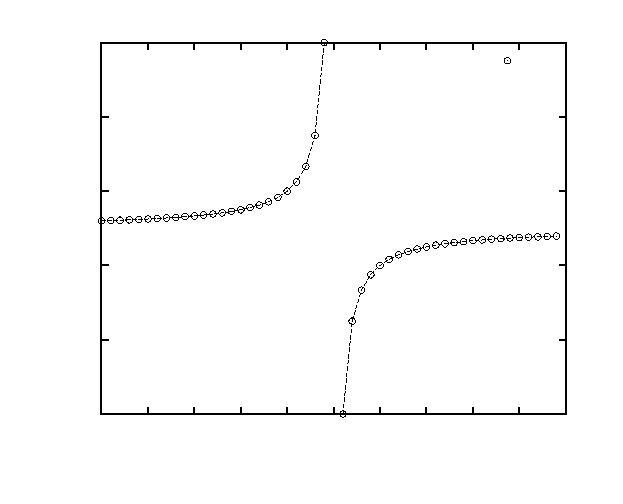
\includegraphics{2-1}}%
    \gplfronttext
  \end{picture}%
\endgroup

	\caption{$x^*$ em função de $\lambda$}
	\label{graph:2-1}
	\end{figure}
\FloatBarrier
\paragraph{}Nos gráficos \ref{graph:2-2-1} a \ref{graph:2-2-3} vemos que o comportamento da iteração depende tanto de $x_0$ como de $\lambda$. Notamos que ocorrem 3 comportamentos característicos: ou a iteração rapidamente diverge ou converge para um valor ou ainda oscila entre dois valores fixos depois de alguns passos.
\FloatBarrier
\begin{figure}
	\hspace{-3.5 cm}
	\begin{subfigure}[!h]{.4\textwidth}
	% GNUPLOT: LaTeX picture with Postscript
\begingroup
  \makeatletter
  \providecommand\color[2][]{%
    \GenericError{(gnuplot) \space\space\space\@spaces}{%
      Package color not loaded in conjunction with
      terminal option `colourtext'%
    }{See the gnuplot documentation for explanation.%
    }{Either use 'blacktext' in gnuplot or load the package
      color.sty in LaTeX.}%
    \renewcommand\color[2][]{}%
  }%
  \providecommand\includegraphics[2][]{%
    \GenericError{(gnuplot) \space\space\space\@spaces}{%
      Package graphicx or graphics not loaded%
    }{See the gnuplot documentation for explanation.%
    }{The gnuplot epslatex terminal needs graphicx.sty or graphics.sty.}%
    \renewcommand\includegraphics[2][]{}%
  }%
  \providecommand\rotatebox[2]{#2}%
  \@ifundefined{ifGPcolor}{%
    \newif\ifGPcolor
    \GPcolorfalse
  }{}%
  \@ifundefined{ifGPblacktext}{%
    \newif\ifGPblacktext
    \GPblacktexttrue
  }{}%
  % define a \g@addto@macro without @ in the name:
  \let\gplgaddtomacro\g@addto@macro
  % define empty templates for all commands taking text:
  \gdef\gplbacktext{}%
  \gdef\gplfronttext{}%
  \makeatother
  \ifGPblacktext
    % no textcolor at all
    \def\colorrgb#1{}%
    \def\colorgray#1{}%
  \else
    % gray or color?
    \ifGPcolor
      \def\colorrgb#1{\color[rgb]{#1}}%
      \def\colorgray#1{\color[gray]{#1}}%
      \expandafter\def\csname LTw\endcsname{\color{white}}%
      \expandafter\def\csname LTb\endcsname{\color{black}}%
      \expandafter\def\csname LTa\endcsname{\color{black}}%
      \expandafter\def\csname LT0\endcsname{\color[rgb]{1,0,0}}%
      \expandafter\def\csname LT1\endcsname{\color[rgb]{0,1,0}}%
      \expandafter\def\csname LT2\endcsname{\color[rgb]{0,0,1}}%
      \expandafter\def\csname LT3\endcsname{\color[rgb]{1,0,1}}%
      \expandafter\def\csname LT4\endcsname{\color[rgb]{0,1,1}}%
      \expandafter\def\csname LT5\endcsname{\color[rgb]{1,1,0}}%
      \expandafter\def\csname LT6\endcsname{\color[rgb]{0,0,0}}%
      \expandafter\def\csname LT7\endcsname{\color[rgb]{1,0.3,0}}%
      \expandafter\def\csname LT8\endcsname{\color[rgb]{0.5,0.5,0.5}}%
    \else
      % gray
      \def\colorrgb#1{\color{black}}%
      \def\colorgray#1{\color[gray]{#1}}%
      \expandafter\def\csname LTw\endcsname{\color{white}}%
      \expandafter\def\csname LTb\endcsname{\color{black}}%
      \expandafter\def\csname LTa\endcsname{\color{black}}%
      \expandafter\def\csname LT0\endcsname{\color{black}}%
      \expandafter\def\csname LT1\endcsname{\color{black}}%
      \expandafter\def\csname LT2\endcsname{\color{black}}%
      \expandafter\def\csname LT3\endcsname{\color{black}}%
      \expandafter\def\csname LT4\endcsname{\color{black}}%
      \expandafter\def\csname LT5\endcsname{\color{black}}%
      \expandafter\def\csname LT6\endcsname{\color{black}}%
      \expandafter\def\csname LT7\endcsname{\color{black}}%
      \expandafter\def\csname LT8\endcsname{\color{black}}%
    \fi
  \fi
  \setlength{\unitlength}{0.0500bp}%
  \begin{picture}(5668.00,4534.00)%
    \gplgaddtomacro\gplbacktext{%
      \csname LTb\endcsname%
      \put(946,968){\makebox(0,0)[r]{\strut{}-1}}%
      \put(946,1628){\makebox(0,0)[r]{\strut{}-0.5}}%
      \put(946,2289){\makebox(0,0)[r]{\strut{} 0}}%
      \put(946,2949){\makebox(0,0)[r]{\strut{} 0.5}}%
      \put(946,3609){\makebox(0,0)[r]{\strut{} 1}}%
      \put(1278,484){\makebox(0,0){\strut{} 0}}%
      \put(2276,484){\makebox(0,0){\strut{} 5}}%
      \put(3274,484){\makebox(0,0){\strut{} 10}}%
      \put(4273,484){\makebox(0,0){\strut{} 15}}%
      \put(5271,484){\makebox(0,0){\strut{} 20}}%
      \put(176,2288){\makebox(0,0){\strut{}$x^{(n)}$}}%
      \put(3174,154){\makebox(0,0){\strut{}n}}%
      \put(3174,4203){\makebox(0,0){\strut{}$x^{(n)} \times n [x_0 = 0.5]$}}%
    }%
    \gplgaddtomacro\gplfronttext{%
      \csname LTb\endcsname%
      \put(2373,1317){\makebox(0,0)[r]{\strut{}$\lambda = -4$}}%
      \csname LTb\endcsname%
      \put(2373,1097){\makebox(0,0)[r]{\strut{}$\lambda = -1.2$}}%
      \csname LTb\endcsname%
      \put(2373,877){\makebox(0,0)[r]{\strut{}$\lambda = -0.4$}}%
      \csname LTb\endcsname%
      \put(4284,1317){\makebox(0,0)[r]{\strut{}$\lambda = 0.4$}}%
      \csname LTb\endcsname%
      \put(4284,1097){\makebox(0,0)[r]{\strut{}$\lambda = 1.2$}}%
      \csname LTb\endcsname%
      \put(4284,877){\makebox(0,0)[r]{\strut{}$\lambda = 5$}}%
    }%
    \gplbacktext
    \put(0,0){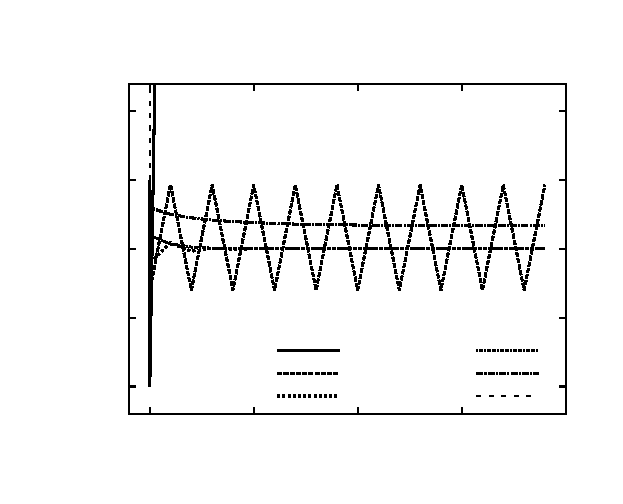
\includegraphics{2-2-1}}%
    \gplfronttext
  \end{picture}%
\endgroup

	\caption{}
	\label{graph:2-2-1}	
	\end{subfigure}
	\hspace{3.0 cm}	
	\begin{subfigure}[h]{.4\textwidth}
		% GNUPLOT: LaTeX picture with Postscript
\begingroup
  \makeatletter
  \providecommand\color[2][]{%
    \GenericError{(gnuplot) \space\space\space\@spaces}{%
      Package color not loaded in conjunction with
      terminal option `colourtext'%
    }{See the gnuplot documentation for explanation.%
    }{Either use 'blacktext' in gnuplot or load the package
      color.sty in LaTeX.}%
    \renewcommand\color[2][]{}%
  }%
  \providecommand\includegraphics[2][]{%
    \GenericError{(gnuplot) \space\space\space\@spaces}{%
      Package graphicx or graphics not loaded%
    }{See the gnuplot documentation for explanation.%
    }{The gnuplot epslatex terminal needs graphicx.sty or graphics.sty.}%
    \renewcommand\includegraphics[2][]{}%
  }%
  \providecommand\rotatebox[2]{#2}%
  \@ifundefined{ifGPcolor}{%
    \newif\ifGPcolor
    \GPcolorfalse
  }{}%
  \@ifundefined{ifGPblacktext}{%
    \newif\ifGPblacktext
    \GPblacktexttrue
  }{}%
  % define a \g@addto@macro without @ in the name:
  \let\gplgaddtomacro\g@addto@macro
  % define empty templates for all commands taking text:
  \gdef\gplbacktext{}%
  \gdef\gplfronttext{}%
  \makeatother
  \ifGPblacktext
    % no textcolor at all
    \def\colorrgb#1{}%
    \def\colorgray#1{}%
  \else
    % gray or color?
    \ifGPcolor
      \def\colorrgb#1{\color[rgb]{#1}}%
      \def\colorgray#1{\color[gray]{#1}}%
      \expandafter\def\csname LTw\endcsname{\color{white}}%
      \expandafter\def\csname LTb\endcsname{\color{black}}%
      \expandafter\def\csname LTa\endcsname{\color{black}}%
      \expandafter\def\csname LT0\endcsname{\color[rgb]{1,0,0}}%
      \expandafter\def\csname LT1\endcsname{\color[rgb]{0,1,0}}%
      \expandafter\def\csname LT2\endcsname{\color[rgb]{0,0,1}}%
      \expandafter\def\csname LT3\endcsname{\color[rgb]{1,0,1}}%
      \expandafter\def\csname LT4\endcsname{\color[rgb]{0,1,1}}%
      \expandafter\def\csname LT5\endcsname{\color[rgb]{1,1,0}}%
      \expandafter\def\csname LT6\endcsname{\color[rgb]{0,0,0}}%
      \expandafter\def\csname LT7\endcsname{\color[rgb]{1,0.3,0}}%
      \expandafter\def\csname LT8\endcsname{\color[rgb]{0.5,0.5,0.5}}%
    \else
      % gray
      \def\colorrgb#1{\color{black}}%
      \def\colorgray#1{\color[gray]{#1}}%
      \expandafter\def\csname LTw\endcsname{\color{white}}%
      \expandafter\def\csname LTb\endcsname{\color{black}}%
      \expandafter\def\csname LTa\endcsname{\color{black}}%
      \expandafter\def\csname LT0\endcsname{\color{black}}%
      \expandafter\def\csname LT1\endcsname{\color{black}}%
      \expandafter\def\csname LT2\endcsname{\color{black}}%
      \expandafter\def\csname LT3\endcsname{\color{black}}%
      \expandafter\def\csname LT4\endcsname{\color{black}}%
      \expandafter\def\csname LT5\endcsname{\color{black}}%
      \expandafter\def\csname LT6\endcsname{\color{black}}%
      \expandafter\def\csname LT7\endcsname{\color{black}}%
      \expandafter\def\csname LT8\endcsname{\color{black}}%
    \fi
  \fi
  \setlength{\unitlength}{0.0500bp}%
  \begin{picture}(5668.00,4534.00)%
    \gplgaddtomacro\gplbacktext{%
      \csname LTb\endcsname%
      \put(946,968){\makebox(0,0)[r]{\strut{}-1}}%
      \put(946,1628){\makebox(0,0)[r]{\strut{}-0.5}}%
      \put(946,2289){\makebox(0,0)[r]{\strut{} 0}}%
      \put(946,2949){\makebox(0,0)[r]{\strut{} 0.5}}%
      \put(946,3609){\makebox(0,0)[r]{\strut{} 1}}%
      \put(1278,484){\makebox(0,0){\strut{} 0}}%
      \put(2276,484){\makebox(0,0){\strut{} 5}}%
      \put(3274,484){\makebox(0,0){\strut{} 10}}%
      \put(4273,484){\makebox(0,0){\strut{} 15}}%
      \put(5271,484){\makebox(0,0){\strut{} 20}}%
      \put(176,2288){\makebox(0,0){\strut{}$x^{(n)}$}}%
      \put(3174,154){\makebox(0,0){\strut{}n}}%
      \put(3174,4203){\makebox(0,0){\strut{}$x^{(n)} \times n [x_0 = 2.0]$}}%
    }%
    \gplgaddtomacro\gplfronttext{%
      \csname LTb\endcsname%
      \put(2373,1317){\makebox(0,0)[r]{\strut{}$\lambda = -4$}}%
      \csname LTb\endcsname%
      \put(2373,1097){\makebox(0,0)[r]{\strut{}$\lambda = -1.2$}}%
      \csname LTb\endcsname%
      \put(2373,877){\makebox(0,0)[r]{\strut{}$\lambda = -0.4$}}%
      \csname LTb\endcsname%
      \put(4284,1317){\makebox(0,0)[r]{\strut{}$\lambda = 0.4$}}%
      \csname LTb\endcsname%
      \put(4284,1097){\makebox(0,0)[r]{\strut{}$\lambda = 1.2$}}%
      \csname LTb\endcsname%
      \put(4284,877){\makebox(0,0)[r]{\strut{}$\lambda = 5$}}%
    }%
    \gplbacktext
    \put(0,0){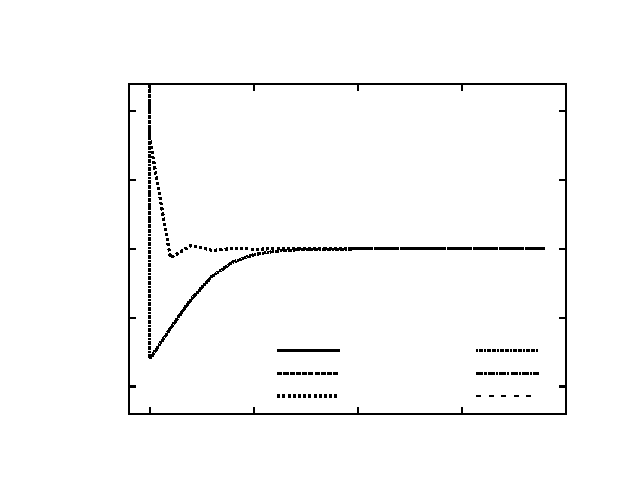
\includegraphics{2-2-2}}%
    \gplfronttext
  \end{picture}%
\endgroup

		\caption{}
		\label{graph:2-2-2}	
	\end{subfigure}

	\begin{subfigure}[h]{.4\textwidth}
		% GNUPLOT: LaTeX picture with Postscript
\begingroup
  \makeatletter
  \providecommand\color[2][]{%
    \GenericError{(gnuplot) \space\space\space\@spaces}{%
      Package color not loaded in conjunction with
      terminal option `colourtext'%
    }{See the gnuplot documentation for explanation.%
    }{Either use 'blacktext' in gnuplot or load the package
      color.sty in LaTeX.}%
    \renewcommand\color[2][]{}%
  }%
  \providecommand\includegraphics[2][]{%
    \GenericError{(gnuplot) \space\space\space\@spaces}{%
      Package graphicx or graphics not loaded%
    }{See the gnuplot documentation for explanation.%
    }{The gnuplot epslatex terminal needs graphicx.sty or graphics.sty.}%
    \renewcommand\includegraphics[2][]{}%
  }%
  \providecommand\rotatebox[2]{#2}%
  \@ifundefined{ifGPcolor}{%
    \newif\ifGPcolor
    \GPcolorfalse
  }{}%
  \@ifundefined{ifGPblacktext}{%
    \newif\ifGPblacktext
    \GPblacktexttrue
  }{}%
  % define a \g@addto@macro without @ in the name:
  \let\gplgaddtomacro\g@addto@macro
  % define empty templates for all commands taking text:
  \gdef\gplbacktext{}%
  \gdef\gplfronttext{}%
  \makeatother
  \ifGPblacktext
    % no textcolor at all
    \def\colorrgb#1{}%
    \def\colorgray#1{}%
  \else
    % gray or color?
    \ifGPcolor
      \def\colorrgb#1{\color[rgb]{#1}}%
      \def\colorgray#1{\color[gray]{#1}}%
      \expandafter\def\csname LTw\endcsname{\color{white}}%
      \expandafter\def\csname LTb\endcsname{\color{black}}%
      \expandafter\def\csname LTa\endcsname{\color{black}}%
      \expandafter\def\csname LT0\endcsname{\color[rgb]{1,0,0}}%
      \expandafter\def\csname LT1\endcsname{\color[rgb]{0,1,0}}%
      \expandafter\def\csname LT2\endcsname{\color[rgb]{0,0,1}}%
      \expandafter\def\csname LT3\endcsname{\color[rgb]{1,0,1}}%
      \expandafter\def\csname LT4\endcsname{\color[rgb]{0,1,1}}%
      \expandafter\def\csname LT5\endcsname{\color[rgb]{1,1,0}}%
      \expandafter\def\csname LT6\endcsname{\color[rgb]{0,0,0}}%
      \expandafter\def\csname LT7\endcsname{\color[rgb]{1,0.3,0}}%
      \expandafter\def\csname LT8\endcsname{\color[rgb]{0.5,0.5,0.5}}%
    \else
      % gray
      \def\colorrgb#1{\color{black}}%
      \def\colorgray#1{\color[gray]{#1}}%
      \expandafter\def\csname LTw\endcsname{\color{white}}%
      \expandafter\def\csname LTb\endcsname{\color{black}}%
      \expandafter\def\csname LTa\endcsname{\color{black}}%
      \expandafter\def\csname LT0\endcsname{\color{black}}%
      \expandafter\def\csname LT1\endcsname{\color{black}}%
      \expandafter\def\csname LT2\endcsname{\color{black}}%
      \expandafter\def\csname LT3\endcsname{\color{black}}%
      \expandafter\def\csname LT4\endcsname{\color{black}}%
      \expandafter\def\csname LT5\endcsname{\color{black}}%
      \expandafter\def\csname LT6\endcsname{\color{black}}%
      \expandafter\def\csname LT7\endcsname{\color{black}}%
      \expandafter\def\csname LT8\endcsname{\color{black}}%
    \fi
  \fi
  \setlength{\unitlength}{0.0500bp}%
  \begin{picture}(5668.00,4534.00)%
    \gplgaddtomacro\gplbacktext{%
      \csname LTb\endcsname%
      \put(946,968){\makebox(0,0)[r]{\strut{}-1}}%
      \put(946,1628){\makebox(0,0)[r]{\strut{}-0.5}}%
      \put(946,2289){\makebox(0,0)[r]{\strut{} 0}}%
      \put(946,2949){\makebox(0,0)[r]{\strut{} 0.5}}%
      \put(946,3609){\makebox(0,0)[r]{\strut{} 1}}%
      \put(1278,484){\makebox(0,0){\strut{} 0}}%
      \put(2276,484){\makebox(0,0){\strut{} 5}}%
      \put(3274,484){\makebox(0,0){\strut{} 10}}%
      \put(4273,484){\makebox(0,0){\strut{} 15}}%
      \put(5271,484){\makebox(0,0){\strut{} 20}}%
      \put(176,2288){\makebox(0,0){\strut{}$x^{(n)}$}}%
      \put(3174,154){\makebox(0,0){\strut{}n}}%
      \put(3174,4203){\makebox(0,0){\strut{}$x^{(n)} \times n [x_0 = -0.5]$}}%
    }%
    \gplgaddtomacro\gplfronttext{%
      \csname LTb\endcsname%
      \put(2373,1317){\makebox(0,0)[r]{\strut{}$\lambda = -4$}}%
      \csname LTb\endcsname%
      \put(2373,1097){\makebox(0,0)[r]{\strut{}$\lambda = -1.2$}}%
      \csname LTb\endcsname%
      \put(2373,877){\makebox(0,0)[r]{\strut{}$\lambda = -0.4$}}%
      \csname LTb\endcsname%
      \put(4284,1317){\makebox(0,0)[r]{\strut{}$\lambda = 0.4$}}%
      \csname LTb\endcsname%
      \put(4284,1097){\makebox(0,0)[r]{\strut{}$\lambda = 1.2$}}%
      \csname LTb\endcsname%
      \put(4284,877){\makebox(0,0)[r]{\strut{}$\lambda = 5$}}%
    }%
    \gplbacktext
    \put(0,0){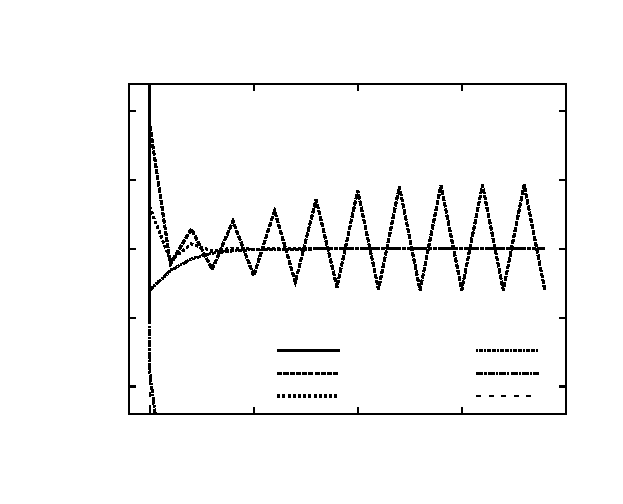
\includegraphics{2-2-3}}%
    \gplfronttext
  \end{picture}%
\endgroup

		\caption{}
		\label{graph:2-2-3}	
	\end{subfigure}
	\caption{Comportamento de $x^{(n)} \times n$ para alguns valores de $x^{(0)}$ e $\lambda$}
\end{figure}
\FloatBarrier
\newpage

\section*{Questão 3}
\paragraph{}Calculamos agora $x^{(n)}_\lambda$ para os 250 primeiros $n$'s com $\lambda \in [0, 4]$ com saltos de 0.001 . O chute inicial usado foi $x_0 = 0.5$. O valor foi escolhido de forma a ser próximo de todos os $x^*$ não triviais e longe o suficiente de 0 para que o processo não convirja necessariamente para a origem. Os primeiros 200 n's são descartados e os 50 últimos plotados no gráfico \ref{graph:3-1}. Para um dado $\lambda$ no intervalo vê-se que depois de algumas iterações(as 200 primeiras descartadas) $x^{(n)}_\lambda$ oscila regularmente dentre $k_\lambda$ valores fixos $x^*_k$. No gráfico \ref{graph:3-2} focamos a região da 'cauda'. Na região da cauda o gráfico muda de comportamento em $\lambda = 3.8$. Essa mudança de comportamento é mostrada em \ref{graph:3-3} e \ref{graph:3-4}.
\paragraph{}Notamos que, como esperado, no intervalo $\lambda \in (0, 3)$ a iteração é convergente e todos os valores de n alto levam $x_n$ perto do ponto fixo $x^*$ único. Para $3 < \lambda < 4 $  nota-se que a iteração diverge mas oscila em torno de um número fixo de valores que é função de $\lambda$, i.e. para um $\lambda$ existe um número $k_\lambda$ de números em torno do qual $x^{(n)}_\lambda$ oscila. Dizemos que o número k é o período da órbita. É interessante notar que no intervalo representado na figura \ref{graph:3-3} o período k parece dobrar regularmente a medida que $\lambda$ aumenta e a figura tem aspecto fractal. A partir de $\lambda = 3.8$ perde-se essa característica de dobra de período e as órbitas parecem ser aleatórias. 
\FloatBarrier
\begin{figure}[!htp]
	\begin{subfigure}[h]{\textwidth}
	\centering
	% GNUPLOT: LaTeX picture with Postscript
\begingroup
  \fontfamily{phv}%
  \selectfont
\definecolor{t}{rgb}{0.5,0.5,0.5}
  \makeatletter
  \providecommand\color[2][]{%
    \GenericError{(gnuplot) \space\space\space\@spaces}{%
      Package color not loaded in conjunction with
      terminal option `colourtext'%
    }{See the gnuplot documentation for explanation.%
    }{Either use 'blacktext' in gnuplot or load the package
      color.sty in LaTeX.}%
    \renewcommand\color[2][]{}%
  }%
  \providecommand\includegraphics[2][]{%
    \GenericError{(gnuplot) \space\space\space\@spaces}{%
      Package graphicx or graphics not loaded%
    }{See the gnuplot documentation for explanation.%
    }{The gnuplot epslatex terminal needs graphicx.sty or graphics.sty.}%
    \renewcommand\includegraphics[2][]{}%
  }%
  \providecommand\rotatebox[2]{#2}%
  \@ifundefined{ifGPcolor}{%
    \newif\ifGPcolor
    \GPcolortrue
  }{}%
  \@ifundefined{ifGPblacktext}{%
    \newif\ifGPblacktext
    \GPblacktextfalse
  }{}%
  % define a \g@addto@macro without @ in the name:
  \let\gplgaddtomacro\g@addto@macro
  % define empty templates for all commands taking text:
  \gdef\gplbacktext{}%
  \gdef\gplfronttext{}%
  \makeatother
  \ifGPblacktext
    % no textcolor at all
    \def\colorrgb#1{}%
    \def\colorgray#1{}%
  \else
    % gray or color?
    \ifGPcolor
      \def\colorrgb#1{\color[rgb]{#1}}%
      \def\colorgray#1{\color[gray]{#1}}%
      \expandafter\def\csname LTw\endcsname{\color{white}}%
      \expandafter\def\csname LTb\endcsname{\color{black}}%
      \expandafter\def\csname LTa\endcsname{\color{black}}%
      \expandafter\def\csname LT0\endcsname{\color[rgb]{1,0,0}}%
      \expandafter\def\csname LT1\endcsname{\color[rgb]{0,1,0}}%
      \expandafter\def\csname LT2\endcsname{\color[rgb]{0,0,1}}%
      \expandafter\def\csname LT3\endcsname{\color[rgb]{1,0,1}}%
      \expandafter\def\csname LT4\endcsname{\color[rgb]{0,1,1}}%
      \expandafter\def\csname LT5\endcsname{\color[rgb]{1,1,0}}%
      \expandafter\def\csname LT6\endcsname{\color[rgb]{0,0,0}}%
      \expandafter\def\csname LT7\endcsname{\color[rgb]{1,0.3,0}}%
      \expandafter\def\csname LT8\endcsname{\color[rgb]{0.5,0.5,0.5}}%
    \else
      % gray
      \def\colorrgb#1{\color{black}}%
      \def\colorgray#1{\color[gray]{#1}}%
      \expandafter\def\csname LTw\endcsname{\color{white}}%
      \expandafter\def\csname LTb\endcsname{\color{black}}%
      \expandafter\def\csname LTa\endcsname{\color{black}}%
      \expandafter\def\csname LT0\endcsname{\color{black}}%
      \expandafter\def\csname LT1\endcsname{\color{black}}%
      \expandafter\def\csname LT2\endcsname{\color{black}}%
      \expandafter\def\csname LT3\endcsname{\color{black}}%
      \expandafter\def\csname LT4\endcsname{\color{black}}%
      \expandafter\def\csname LT5\endcsname{\color{black}}%
      \expandafter\def\csname LT6\endcsname{\color{black}}%
      \expandafter\def\csname LT7\endcsname{\color{black}}%
      \expandafter\def\csname LT8\endcsname{\color{black}}%
    \fi
  \fi
  \setlength{\unitlength}{0.0500bp}%
  \begin{picture}(7936.00,4534.00)%
    \gplgaddtomacro\gplbacktext{%
      \csname LTb\endcsname%
      \put(774,901){\makebox(0,0)[r]{\strut{} 0}}%
      \put(774,1552){\makebox(0,0)[r]{\strut{} 0.2}}%
      \put(774,2203){\makebox(0,0)[r]{\strut{} 0.4}}%
      \put(774,2853){\makebox(0,0)[r]{\strut{} 0.6}}%
      \put(774,3504){\makebox(0,0)[r]{\strut{} 0.8}}%
      \put(774,4154){\makebox(0,0)[r]{\strut{} 1}}%
      \put(882,396){\makebox(0,0){\strut{} 0}}%
      \put(1723,396){\makebox(0,0){\strut{} 0.5}}%
      \put(2564,396){\makebox(0,0){\strut{} 1}}%
      \put(3405,396){\makebox(0,0){\strut{} 1.5}}%
      \put(4247,396){\makebox(0,0){\strut{} 2}}%
      \put(5088,396){\makebox(0,0){\strut{} 2.5}}%
      \put(5929,396){\makebox(0,0){\strut{} 3}}%
      \put(6770,396){\makebox(0,0){\strut{} 3.5}}%
      \put(7611,396){\makebox(0,0){\strut{} 4}}%
      \put(144,2446){\makebox(0,0){\strut{}$x^*_k$}}%
      \put(4246,126){\makebox(0,0){\strut{}$\lambda$}}%
    }%
    \gplgaddtomacro\gplfronttext{%
    }%
    \gplbacktext
    \put(0,0){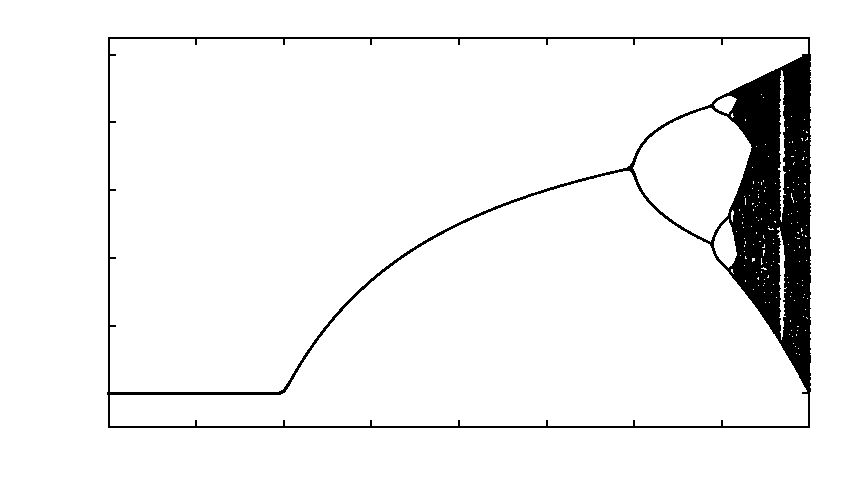
\includegraphics{3-2}}%
    \gplfronttext
  \end{picture}%
\endgroup

	\caption{}
	\label{graph:3-1}
	\end{subfigure}	
	
	\begin{subfigure}[h]{\textwidth}
	\centering	
	% GNUPLOT: LaTeX picture with Postscript
\begingroup
  \fontfamily{phv}%
  \selectfont
\definecolor{t}{rgb}{0.5,0.5,0.5}
  \makeatletter
  \providecommand\color[2][]{%
    \GenericError{(gnuplot) \space\space\space\@spaces}{%
      Package color not loaded in conjunction with
      terminal option `colourtext'%
    }{See the gnuplot documentation for explanation.%
    }{Either use 'blacktext' in gnuplot or load the package
      color.sty in LaTeX.}%
    \renewcommand\color[2][]{}%
  }%
  \providecommand\includegraphics[2][]{%
    \GenericError{(gnuplot) \space\space\space\@spaces}{%
      Package graphicx or graphics not loaded%
    }{See the gnuplot documentation for explanation.%
    }{The gnuplot epslatex terminal needs graphicx.sty or graphics.sty.}%
    \renewcommand\includegraphics[2][]{}%
  }%
  \providecommand\rotatebox[2]{#2}%
  \@ifundefined{ifGPcolor}{%
    \newif\ifGPcolor
    \GPcolortrue
  }{}%
  \@ifundefined{ifGPblacktext}{%
    \newif\ifGPblacktext
    \GPblacktextfalse
  }{}%
  % define a \g@addto@macro without @ in the name:
  \let\gplgaddtomacro\g@addto@macro
  % define empty templates for all commands taking text:
  \gdef\gplbacktext{}%
  \gdef\gplfronttext{}%
  \makeatother
  \ifGPblacktext
    % no textcolor at all
    \def\colorrgb#1{}%
    \def\colorgray#1{}%
  \else
    % gray or color?
    \ifGPcolor
      \def\colorrgb#1{\color[rgb]{#1}}%
      \def\colorgray#1{\color[gray]{#1}}%
      \expandafter\def\csname LTw\endcsname{\color{white}}%
      \expandafter\def\csname LTb\endcsname{\color{black}}%
      \expandafter\def\csname LTa\endcsname{\color{black}}%
      \expandafter\def\csname LT0\endcsname{\color[rgb]{1,0,0}}%
      \expandafter\def\csname LT1\endcsname{\color[rgb]{0,1,0}}%
      \expandafter\def\csname LT2\endcsname{\color[rgb]{0,0,1}}%
      \expandafter\def\csname LT3\endcsname{\color[rgb]{1,0,1}}%
      \expandafter\def\csname LT4\endcsname{\color[rgb]{0,1,1}}%
      \expandafter\def\csname LT5\endcsname{\color[rgb]{1,1,0}}%
      \expandafter\def\csname LT6\endcsname{\color[rgb]{0,0,0}}%
      \expandafter\def\csname LT7\endcsname{\color[rgb]{1,0.3,0}}%
      \expandafter\def\csname LT8\endcsname{\color[rgb]{0.5,0.5,0.5}}%
    \else
      % gray
      \def\colorrgb#1{\color{black}}%
      \def\colorgray#1{\color[gray]{#1}}%
      \expandafter\def\csname LTw\endcsname{\color{white}}%
      \expandafter\def\csname LTb\endcsname{\color{black}}%
      \expandafter\def\csname LTa\endcsname{\color{black}}%
      \expandafter\def\csname LT0\endcsname{\color{black}}%
      \expandafter\def\csname LT1\endcsname{\color{black}}%
      \expandafter\def\csname LT2\endcsname{\color{black}}%
      \expandafter\def\csname LT3\endcsname{\color{black}}%
      \expandafter\def\csname LT4\endcsname{\color{black}}%
      \expandafter\def\csname LT5\endcsname{\color{black}}%
      \expandafter\def\csname LT6\endcsname{\color{black}}%
      \expandafter\def\csname LT7\endcsname{\color{black}}%
      \expandafter\def\csname LT8\endcsname{\color{black}}%
    \fi
  \fi
  \setlength{\unitlength}{0.0500bp}%
  \begin{picture}(7936.00,4534.00)%
    \gplgaddtomacro\gplbacktext{%
      \csname LTb\endcsname%
      \put(774,576){\makebox(0,0)[r]{\strut{} 0}}%
      \put(774,950){\makebox(0,0)[r]{\strut{} 0.1}}%
      \put(774,1324){\makebox(0,0)[r]{\strut{} 0.2}}%
      \put(774,1698){\makebox(0,0)[r]{\strut{} 0.3}}%
      \put(774,2072){\makebox(0,0)[r]{\strut{} 0.4}}%
      \put(774,2447){\makebox(0,0)[r]{\strut{} 0.5}}%
      \put(774,2821){\makebox(0,0)[r]{\strut{} 0.6}}%
      \put(774,3195){\makebox(0,0)[r]{\strut{} 0.7}}%
      \put(774,3569){\makebox(0,0)[r]{\strut{} 0.8}}%
      \put(774,3943){\makebox(0,0)[r]{\strut{} 0.9}}%
      \put(774,4317){\makebox(0,0)[r]{\strut{} 1}}%
      \put(882,396){\makebox(0,0){\strut{} 3}}%
      \put(1555,396){\makebox(0,0){\strut{} 3.1}}%
      \put(2228,396){\makebox(0,0){\strut{} 3.2}}%
      \put(2901,396){\makebox(0,0){\strut{} 3.3}}%
      \put(3574,396){\makebox(0,0){\strut{} 3.4}}%
      \put(4247,396){\makebox(0,0){\strut{} 3.5}}%
      \put(4919,396){\makebox(0,0){\strut{} 3.6}}%
      \put(5592,396){\makebox(0,0){\strut{} 3.7}}%
      \put(6265,396){\makebox(0,0){\strut{} 3.8}}%
      \put(6938,396){\makebox(0,0){\strut{} 3.9}}%
      \put(7611,396){\makebox(0,0){\strut{} 4}}%
      \put(144,2446){\makebox(0,0){\strut{}$x^*_k(\lambda)$}}%
      \put(4246,126){\makebox(0,0){\strut{}$\lambda$}}%
    }%
    \gplgaddtomacro\gplfronttext{%
    }%
    \gplbacktext
    \put(0,0){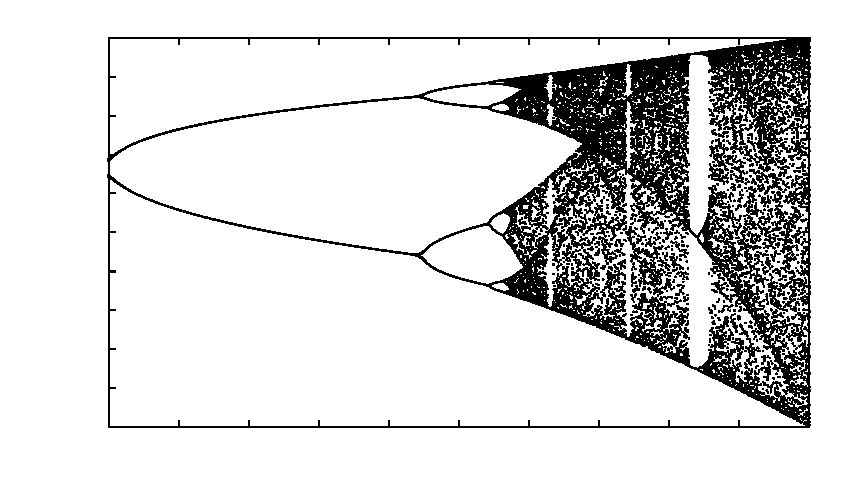
\includegraphics{3-1}}%
    \gplfronttext
  \end{picture}%
\endgroup

	\caption{foco na cauda}
	\label{graph:3-2}	
	\end{subfigure}	
	\caption{Mapa Logístico}
\end{figure}
\FloatBarrier
\FloatBarrier
\begin{figure}[!htp]
	\begin{subfigure}[h]{0.4\textwidth}
	\centering
	% GNUPLOT: LaTeX picture with Postscript
\begingroup
  \fontfamily{phv}%
  \selectfont
\definecolor{t}{rgb}{0.5,0.5,0.5}
  \makeatletter
  \providecommand\color[2][]{%
    \GenericError{(gnuplot) \space\space\space\@spaces}{%
      Package color not loaded in conjunction with
      terminal option `colourtext'%
    }{See the gnuplot documentation for explanation.%
    }{Either use 'blacktext' in gnuplot or load the package
      color.sty in LaTeX.}%
    \renewcommand\color[2][]{}%
  }%
  \providecommand\includegraphics[2][]{%
    \GenericError{(gnuplot) \space\space\space\@spaces}{%
      Package graphicx or graphics not loaded%
    }{See the gnuplot documentation for explanation.%
    }{The gnuplot epslatex terminal needs graphicx.sty or graphics.sty.}%
    \renewcommand\includegraphics[2][]{}%
  }%
  \providecommand\rotatebox[2]{#2}%
  \@ifundefined{ifGPcolor}{%
    \newif\ifGPcolor
    \GPcolortrue
  }{}%
  \@ifundefined{ifGPblacktext}{%
    \newif\ifGPblacktext
    \GPblacktextfalse
  }{}%
  % define a \g@addto@macro without @ in the name:
  \let\gplgaddtomacro\g@addto@macro
  % define empty templates for all commands taking text:
  \gdef\gplbacktext{}%
  \gdef\gplfronttext{}%
  \makeatother
  \ifGPblacktext
    % no textcolor at all
    \def\colorrgb#1{}%
    \def\colorgray#1{}%
  \else
    % gray or color?
    \ifGPcolor
      \def\colorrgb#1{\color[rgb]{#1}}%
      \def\colorgray#1{\color[gray]{#1}}%
      \expandafter\def\csname LTw\endcsname{\color{white}}%
      \expandafter\def\csname LTb\endcsname{\color{black}}%
      \expandafter\def\csname LTa\endcsname{\color{black}}%
      \expandafter\def\csname LT0\endcsname{\color[rgb]{1,0,0}}%
      \expandafter\def\csname LT1\endcsname{\color[rgb]{0,1,0}}%
      \expandafter\def\csname LT2\endcsname{\color[rgb]{0,0,1}}%
      \expandafter\def\csname LT3\endcsname{\color[rgb]{1,0,1}}%
      \expandafter\def\csname LT4\endcsname{\color[rgb]{0,1,1}}%
      \expandafter\def\csname LT5\endcsname{\color[rgb]{1,1,0}}%
      \expandafter\def\csname LT6\endcsname{\color[rgb]{0,0,0}}%
      \expandafter\def\csname LT7\endcsname{\color[rgb]{1,0.3,0}}%
      \expandafter\def\csname LT8\endcsname{\color[rgb]{0.5,0.5,0.5}}%
    \else
      % gray
      \def\colorrgb#1{\color{black}}%
      \def\colorgray#1{\color[gray]{#1}}%
      \expandafter\def\csname LTw\endcsname{\color{white}}%
      \expandafter\def\csname LTb\endcsname{\color{black}}%
      \expandafter\def\csname LTa\endcsname{\color{black}}%
      \expandafter\def\csname LT0\endcsname{\color{black}}%
      \expandafter\def\csname LT1\endcsname{\color{black}}%
      \expandafter\def\csname LT2\endcsname{\color{black}}%
      \expandafter\def\csname LT3\endcsname{\color{black}}%
      \expandafter\def\csname LT4\endcsname{\color{black}}%
      \expandafter\def\csname LT5\endcsname{\color{black}}%
      \expandafter\def\csname LT6\endcsname{\color{black}}%
      \expandafter\def\csname LT7\endcsname{\color{black}}%
      \expandafter\def\csname LT8\endcsname{\color{black}}%
    \fi
  \fi
  \setlength{\unitlength}{0.0500bp}%
  \begin{picture}(7936.00,4534.00)%
    \gplgaddtomacro\gplbacktext{%
      \csname LTb\endcsname%
      \put(774,576){\makebox(0,0)[r]{\strut{} 0.2}}%
      \put(774,1044){\makebox(0,0)[r]{\strut{} 0.3}}%
      \put(774,1511){\makebox(0,0)[r]{\strut{} 0.4}}%
      \put(774,1979){\makebox(0,0)[r]{\strut{} 0.5}}%
      \put(774,2447){\makebox(0,0)[r]{\strut{} 0.6}}%
      \put(774,2914){\makebox(0,0)[r]{\strut{} 0.7}}%
      \put(774,3382){\makebox(0,0)[r]{\strut{} 0.8}}%
      \put(774,3849){\makebox(0,0)[r]{\strut{} 0.9}}%
      \put(774,4317){\makebox(0,0)[r]{\strut{} 1}}%
      \put(882,396){\makebox(0,0){\strut{} 3.4}}%
      \put(1723,396){\makebox(0,0){\strut{} 3.45}}%
      \put(2564,396){\makebox(0,0){\strut{} 3.5}}%
      \put(3405,396){\makebox(0,0){\strut{} 3.55}}%
      \put(4246,396){\makebox(0,0){\strut{} 3.6}}%
      \put(5088,396){\makebox(0,0){\strut{} 3.65}}%
      \put(5929,396){\makebox(0,0){\strut{} 3.7}}%
      \put(6770,396){\makebox(0,0){\strut{} 3.75}}%
      \put(7611,396){\makebox(0,0){\strut{} 3.8}}%
      \put(144,2446){\makebox(0,0){\strut{}$x^*_k$}}%
      \put(4246,126){\makebox(0,0){\strut{}$\lambda$}}%
    }%
    \gplgaddtomacro\gplfronttext{%
    }%
    \gplbacktext
    \put(0,0){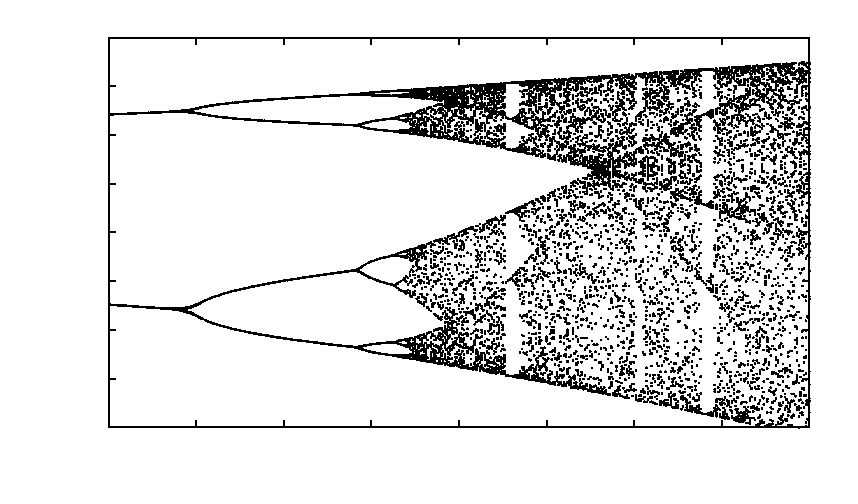
\includegraphics{3-3}}%
    \gplfronttext
  \end{picture}%
\endgroup

	\caption{}
	\label{graph:3-3}
	\end{subfigure}	

	\begin{subfigure}[h]{\textwidth}
	\centering	
	% GNUPLOT: LaTeX picture with Postscript
\begingroup
  \fontfamily{phv}%
  \selectfont
\definecolor{t}{rgb}{0.5,0.5,0.5}
  \makeatletter
  \providecommand\color[2][]{%
    \GenericError{(gnuplot) \space\space\space\@spaces}{%
      Package color not loaded in conjunction with
      terminal option `colourtext'%
    }{See the gnuplot documentation for explanation.%
    }{Either use 'blacktext' in gnuplot or load the package
      color.sty in LaTeX.}%
    \renewcommand\color[2][]{}%
  }%
  \providecommand\includegraphics[2][]{%
    \GenericError{(gnuplot) \space\space\space\@spaces}{%
      Package graphicx or graphics not loaded%
    }{See the gnuplot documentation for explanation.%
    }{The gnuplot epslatex terminal needs graphicx.sty or graphics.sty.}%
    \renewcommand\includegraphics[2][]{}%
  }%
  \providecommand\rotatebox[2]{#2}%
  \@ifundefined{ifGPcolor}{%
    \newif\ifGPcolor
    \GPcolortrue
  }{}%
  \@ifundefined{ifGPblacktext}{%
    \newif\ifGPblacktext
    \GPblacktextfalse
  }{}%
  % define a \g@addto@macro without @ in the name:
  \let\gplgaddtomacro\g@addto@macro
  % define empty templates for all commands taking text:
  \gdef\gplbacktext{}%
  \gdef\gplfronttext{}%
  \makeatother
  \ifGPblacktext
    % no textcolor at all
    \def\colorrgb#1{}%
    \def\colorgray#1{}%
  \else
    % gray or color?
    \ifGPcolor
      \def\colorrgb#1{\color[rgb]{#1}}%
      \def\colorgray#1{\color[gray]{#1}}%
      \expandafter\def\csname LTw\endcsname{\color{white}}%
      \expandafter\def\csname LTb\endcsname{\color{black}}%
      \expandafter\def\csname LTa\endcsname{\color{black}}%
      \expandafter\def\csname LT0\endcsname{\color[rgb]{1,0,0}}%
      \expandafter\def\csname LT1\endcsname{\color[rgb]{0,1,0}}%
      \expandafter\def\csname LT2\endcsname{\color[rgb]{0,0,1}}%
      \expandafter\def\csname LT3\endcsname{\color[rgb]{1,0,1}}%
      \expandafter\def\csname LT4\endcsname{\color[rgb]{0,1,1}}%
      \expandafter\def\csname LT5\endcsname{\color[rgb]{1,1,0}}%
      \expandafter\def\csname LT6\endcsname{\color[rgb]{0,0,0}}%
      \expandafter\def\csname LT7\endcsname{\color[rgb]{1,0.3,0}}%
      \expandafter\def\csname LT8\endcsname{\color[rgb]{0.5,0.5,0.5}}%
    \else
      % gray
      \def\colorrgb#1{\color{black}}%
      \def\colorgray#1{\color[gray]{#1}}%
      \expandafter\def\csname LTw\endcsname{\color{white}}%
      \expandafter\def\csname LTb\endcsname{\color{black}}%
      \expandafter\def\csname LTa\endcsname{\color{black}}%
      \expandafter\def\csname LT0\endcsname{\color{black}}%
      \expandafter\def\csname LT1\endcsname{\color{black}}%
      \expandafter\def\csname LT2\endcsname{\color{black}}%
      \expandafter\def\csname LT3\endcsname{\color{black}}%
      \expandafter\def\csname LT4\endcsname{\color{black}}%
      \expandafter\def\csname LT5\endcsname{\color{black}}%
      \expandafter\def\csname LT6\endcsname{\color{black}}%
      \expandafter\def\csname LT7\endcsname{\color{black}}%
      \expandafter\def\csname LT8\endcsname{\color{black}}%
    \fi
  \fi
  \setlength{\unitlength}{0.0500bp}%
  \begin{picture}(7936.00,4534.00)%
    \gplgaddtomacro\gplbacktext{%
      \csname LTb\endcsname%
      \put(774,576){\makebox(0,0)[r]{\strut{} 0}}%
      \put(774,1324){\makebox(0,0)[r]{\strut{} 0.2}}%
      \put(774,2072){\makebox(0,0)[r]{\strut{} 0.4}}%
      \put(774,2821){\makebox(0,0)[r]{\strut{} 0.6}}%
      \put(774,3569){\makebox(0,0)[r]{\strut{} 0.8}}%
      \put(774,4317){\makebox(0,0)[r]{\strut{} 1}}%
      \put(882,396){\makebox(0,0){\strut{} 3.8}}%
      \put(2564,396){\makebox(0,0){\strut{} 3.85}}%
      \put(4246,396){\makebox(0,0){\strut{} 3.9}}%
      \put(5929,396){\makebox(0,0){\strut{} 3.95}}%
      \put(7611,396){\makebox(0,0){\strut{} 4}}%
      \put(144,2446){\makebox(0,0){\strut{}$x^*_k$}}%
      \put(4246,126){\makebox(0,0){\strut{}$\lambda$}}%
    }%
    \gplgaddtomacro\gplfronttext{%
    }%
    \gplbacktext
    \put(0,0){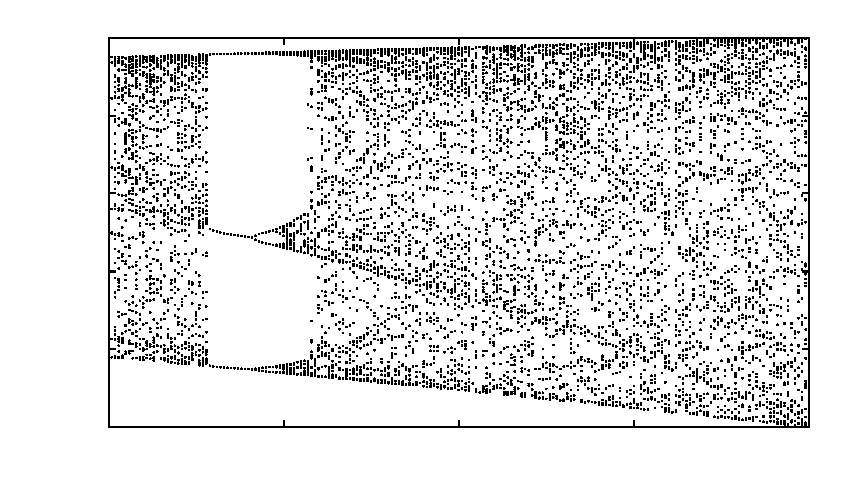
\includegraphics{3-4}}%
    \gplfronttext
  \end{picture}%
\endgroup

	\caption{}
	\label{graph:3-4}	
	\end{subfigure}	
	\caption{Mapa Logístico - mudança no comportamento da cauda}
\end{figure}
\FloatBarrier

\section*{Questão 4}
\paragraph{}Estudamos agora a relação de $\lambda$ com o período $k$ correspondente. Isso é feito descartando-se as primeiras 200 iterações e tomando-se $x_{find} = x^{(201)}$ como um valor a ser procurado nas próximas iterações. As iterações são contadas então até que esse valor $x_{find}$ se repita. Nota-se experimentalmente que  os valores de uma órbita que parecem se repetir no gráfico são próximos mas não necessariamente os mesmos. Damos portanto uma margem de erro para considerarmos quando um mesmo valor se repetiu. Em nossa rotina essa margem de erro é de 0.01. Isto é: dado um $x_{find} = x^{(201)}$ quando $|x_{find} - x^{(n)} < 0.01|$ paramos as iterações e dizemos que o período $k$ da órbita achada $n -201$. O algoritmo deve funcionar bem para as órbitas de baixos períodos nas quais os $x_k^*$ estão distantes. Para as órbitas de altos períodos vemos que os $x_k^*$'s podem estar muito próximos e nossa avaliação falha. Apesar disso o algoritmo será usado porque as órbitas mais frequentes, e portanto de maior interesse, são aquelas de períodos mais curtos para os quais o método funciona.
\paragraph{} É claro da questão 3 que todos os primeiros $\lambda$'s possuem órbitas baixas, a riqueza se encontra nas altas órbitas. Para melhor observar esse comportamento os gráficos \ref{graph:4-1} e \ref{graph:4-2}  apresentam separadamente as órbitas de altos e baixos períodos. O gráfico \ref{graph:4-3} mostra a frequência $f(k)$ de um órbita de período $k$ em função de $k$. Os primeiros termos, órbitas de alta frequência, são omitidos para que se possa observar o que acontece melhor na cauda no gráfico. Em particular obtemos:
	\begin{displaymath}
		\begin{tabular}{ll}
			para $k = 2$ & $f(k) = 463$ \\
			para $k = 5$ & $f(k) = 21$ \\		
		\end{tabular}			
	\end{displaymath}
	
\paragraph{}Os k's acimas foram calculados usando $\lambda$ em incrementos de 0.001 e os gráficos apresentados com incrementos de 0.01. A escolha foi feita para permitir uma melhor avaliação quantitativa das frequências e permitir uma melhor visualização dos dados.
	\FloatBarrier	
	
	\begin{figure}[!htp]
	\centering
	% GNUPLOT: LaTeX picture with Postscript
\begingroup
  \makeatletter
  \providecommand\color[2][]{%
    \GenericError{(gnuplot) \space\space\space\@spaces}{%
      Package color not loaded in conjunction with
      terminal option `colourtext'%
    }{See the gnuplot documentation for explanation.%
    }{Either use 'blacktext' in gnuplot or load the package
      color.sty in LaTeX.}%
    \renewcommand\color[2][]{}%
  }%
  \providecommand\includegraphics[2][]{%
    \GenericError{(gnuplot) \space\space\space\@spaces}{%
      Package graphicx or graphics not loaded%
    }{See the gnuplot documentation for explanation.%
    }{The gnuplot epslatex terminal needs graphicx.sty or graphics.sty.}%
    \renewcommand\includegraphics[2][]{}%
  }%
  \providecommand\rotatebox[2]{#2}%
  \@ifundefined{ifGPcolor}{%
    \newif\ifGPcolor
    \GPcolorfalse
  }{}%
  \@ifundefined{ifGPblacktext}{%
    \newif\ifGPblacktext
    \GPblacktexttrue
  }{}%
  % define a \g@addto@macro without @ in the name:
  \let\gplgaddtomacro\g@addto@macro
  % define empty templates for all commands taking text:
  \gdef\gplbacktext{}%
  \gdef\gplfronttext{}%
  \makeatother
  \ifGPblacktext
    % no textcolor at all
    \def\colorrgb#1{}%
    \def\colorgray#1{}%
  \else
    % gray or color?
    \ifGPcolor
      \def\colorrgb#1{\color[rgb]{#1}}%
      \def\colorgray#1{\color[gray]{#1}}%
      \expandafter\def\csname LTw\endcsname{\color{white}}%
      \expandafter\def\csname LTb\endcsname{\color{black}}%
      \expandafter\def\csname LTa\endcsname{\color{black}}%
      \expandafter\def\csname LT0\endcsname{\color[rgb]{1,0,0}}%
      \expandafter\def\csname LT1\endcsname{\color[rgb]{0,1,0}}%
      \expandafter\def\csname LT2\endcsname{\color[rgb]{0,0,1}}%
      \expandafter\def\csname LT3\endcsname{\color[rgb]{1,0,1}}%
      \expandafter\def\csname LT4\endcsname{\color[rgb]{0,1,1}}%
      \expandafter\def\csname LT5\endcsname{\color[rgb]{1,1,0}}%
      \expandafter\def\csname LT6\endcsname{\color[rgb]{0,0,0}}%
      \expandafter\def\csname LT7\endcsname{\color[rgb]{1,0.3,0}}%
      \expandafter\def\csname LT8\endcsname{\color[rgb]{0.5,0.5,0.5}}%
    \else
      % gray
      \def\colorrgb#1{\color{black}}%
      \def\colorgray#1{\color[gray]{#1}}%
      \expandafter\def\csname LTw\endcsname{\color{white}}%
      \expandafter\def\csname LTb\endcsname{\color{black}}%
      \expandafter\def\csname LTa\endcsname{\color{black}}%
      \expandafter\def\csname LT0\endcsname{\color{black}}%
      \expandafter\def\csname LT1\endcsname{\color{black}}%
      \expandafter\def\csname LT2\endcsname{\color{black}}%
      \expandafter\def\csname LT3\endcsname{\color{black}}%
      \expandafter\def\csname LT4\endcsname{\color{black}}%
      \expandafter\def\csname LT5\endcsname{\color{black}}%
      \expandafter\def\csname LT6\endcsname{\color{black}}%
      \expandafter\def\csname LT7\endcsname{\color{black}}%
      \expandafter\def\csname LT8\endcsname{\color{black}}%
    \fi
  \fi
  \setlength{\unitlength}{0.0500bp}%
  \begin{picture}(7936.00,5102.00)%
    \gplgaddtomacro\gplbacktext{%
      \csname LTb\endcsname%
      \put(946,704){\makebox(0,0)[r]{\strut{} 0}}%
      \put(946,1117){\makebox(0,0)[r]{\strut{} 50}}%
      \put(946,1531){\makebox(0,0)[r]{\strut{} 100}}%
      \put(946,1944){\makebox(0,0)[r]{\strut{} 150}}%
      \put(946,2357){\makebox(0,0)[r]{\strut{} 200}}%
      \put(946,2771){\makebox(0,0)[r]{\strut{} 250}}%
      \put(946,3184){\makebox(0,0)[r]{\strut{} 300}}%
      \put(946,3597){\makebox(0,0)[r]{\strut{} 350}}%
      \put(946,4010){\makebox(0,0)[r]{\strut{} 400}}%
      \put(946,4424){\makebox(0,0)[r]{\strut{} 450}}%
      \put(946,4837){\makebox(0,0)[r]{\strut{} 500}}%
      \put(1078,484){\makebox(0,0){\strut{} 0}}%
      \put(1796,484){\makebox(0,0){\strut{} 20}}%
      \put(2514,484){\makebox(0,0){\strut{} 40}}%
      \put(3232,484){\makebox(0,0){\strut{} 60}}%
      \put(3950,484){\makebox(0,0){\strut{} 80}}%
      \put(4667,484){\makebox(0,0){\strut{} 100}}%
      \put(5385,484){\makebox(0,0){\strut{} 120}}%
      \put(6103,484){\makebox(0,0){\strut{} 140}}%
      \put(6821,484){\makebox(0,0){\strut{} 160}}%
      \put(7539,484){\makebox(0,0){\strut{} 180}}%
      \put(176,2770){\rotatebox{-270}{\makebox(0,0){\strut{}luminosidade}}}%
      \put(4308,154){\makebox(0,0){\strut{}$\theta(º)$}}%
    }%
    \gplgaddtomacro\gplfronttext{%
      \csname LTb\endcsname%
      \put(5267,4664){\makebox(0,0)[r]{\strut{}placa $\frac{\lambda}{4}$ em 0º}}%
      \csname LTb\endcsname%
      \put(5267,4444){\makebox(0,0)[r]{\strut{}              em 90º}}%
      \csname LTb\endcsname%
      \put(5267,4224){\makebox(0,0)[r]{\strut{}polarizador em 45º}}%
    }%
    \gplbacktext
    \put(0,0){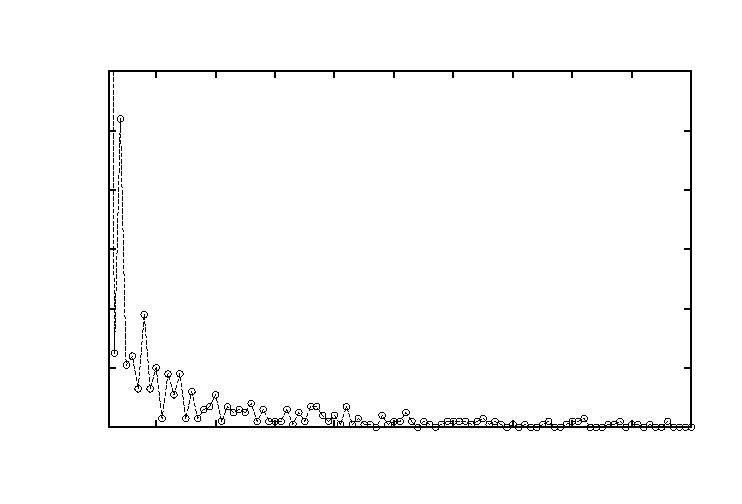
\includegraphics{4-3}}%
    \gplfronttext
  \end{picture}%
\endgroup

	\caption{}
	\label{graph:4-3}
	\end{figure}
	 \FloatBarrier	
	\FloatBarrier	
\begin{figure}
	\hspace{-4.0 cm}
	\begin{subfigure}[!htp]{0.5\textwidth}
	% GNUPLOT: LaTeX picture with Postscript
\begingroup
  \fontfamily{phv}%
  \selectfont
\definecolor{t}{rgb}{0.5,0.5,0.5}
  \makeatletter
  \providecommand\color[2][]{%
    \GenericError{(gnuplot) \space\space\space\@spaces}{%
      Package color not loaded in conjunction with
      terminal option `colourtext'%
    }{See the gnuplot documentation for explanation.%
    }{Either use 'blacktext' in gnuplot or load the package
      color.sty in LaTeX.}%
    \renewcommand\color[2][]{}%
  }%
  \providecommand\includegraphics[2][]{%
    \GenericError{(gnuplot) \space\space\space\@spaces}{%
      Package graphicx or graphics not loaded%
    }{See the gnuplot documentation for explanation.%
    }{The gnuplot epslatex terminal needs graphicx.sty or graphics.sty.}%
    \renewcommand\includegraphics[2][]{}%
  }%
  \providecommand\rotatebox[2]{#2}%
  \@ifundefined{ifGPcolor}{%
    \newif\ifGPcolor
    \GPcolortrue
  }{}%
  \@ifundefined{ifGPblacktext}{%
    \newif\ifGPblacktext
    \GPblacktextfalse
  }{}%
  % define a \g@addto@macro without @ in the name:
  \let\gplgaddtomacro\g@addto@macro
  % define empty templates for all commands taking text:
  \gdef\gplbacktext{}%
  \gdef\gplfronttext{}%
  \makeatother
  \ifGPblacktext
    % no textcolor at all
    \def\colorrgb#1{}%
    \def\colorgray#1{}%
  \else
    % gray or color?
    \ifGPcolor
      \def\colorrgb#1{\color[rgb]{#1}}%
      \def\colorgray#1{\color[gray]{#1}}%
      \expandafter\def\csname LTw\endcsname{\color{white}}%
      \expandafter\def\csname LTb\endcsname{\color{black}}%
      \expandafter\def\csname LTa\endcsname{\color{black}}%
      \expandafter\def\csname LT0\endcsname{\color[rgb]{1,0,0}}%
      \expandafter\def\csname LT1\endcsname{\color[rgb]{0,1,0}}%
      \expandafter\def\csname LT2\endcsname{\color[rgb]{0,0,1}}%
      \expandafter\def\csname LT3\endcsname{\color[rgb]{1,0,1}}%
      \expandafter\def\csname LT4\endcsname{\color[rgb]{0,1,1}}%
      \expandafter\def\csname LT5\endcsname{\color[rgb]{1,1,0}}%
      \expandafter\def\csname LT6\endcsname{\color[rgb]{0,0,0}}%
      \expandafter\def\csname LT7\endcsname{\color[rgb]{1,0.3,0}}%
      \expandafter\def\csname LT8\endcsname{\color[rgb]{0.5,0.5,0.5}}%
    \else
      % gray
      \def\colorrgb#1{\color{black}}%
      \def\colorgray#1{\color[gray]{#1}}%
      \expandafter\def\csname LTw\endcsname{\color{white}}%
      \expandafter\def\csname LTb\endcsname{\color{black}}%
      \expandafter\def\csname LTa\endcsname{\color{black}}%
      \expandafter\def\csname LT0\endcsname{\color{black}}%
      \expandafter\def\csname LT1\endcsname{\color{black}}%
      \expandafter\def\csname LT2\endcsname{\color{black}}%
      \expandafter\def\csname LT3\endcsname{\color{black}}%
      \expandafter\def\csname LT4\endcsname{\color{black}}%
      \expandafter\def\csname LT5\endcsname{\color{black}}%
      \expandafter\def\csname LT6\endcsname{\color{black}}%
      \expandafter\def\csname LT7\endcsname{\color{black}}%
      \expandafter\def\csname LT8\endcsname{\color{black}}%
    \fi
  \fi
  \setlength{\unitlength}{0.0500bp}%
  \begin{picture}(5668.00,3968.00)%
    \gplgaddtomacro\gplbacktext{%
      \csname LTb\endcsname%
      \put(774,576){\makebox(0,0)[r]{\strut{} 1}}%
      \put(774,1051){\makebox(0,0)[r]{\strut{} 1.5}}%
      \put(774,1526){\makebox(0,0)[r]{\strut{} 2}}%
      \put(774,2002){\makebox(0,0)[r]{\strut{} 2.5}}%
      \put(774,2477){\makebox(0,0)[r]{\strut{} 3}}%
      \put(774,2952){\makebox(0,0)[r]{\strut{} 3.5}}%
      \put(774,3427){\makebox(0,0)[r]{\strut{} 4}}%
      \put(882,396){\makebox(0,0){\strut{} 0}}%
      \put(1519,396){\makebox(0,0){\strut{} 0.5}}%
      \put(2157,396){\makebox(0,0){\strut{} 1}}%
      \put(2794,396){\makebox(0,0){\strut{} 1.5}}%
      \put(3431,396){\makebox(0,0){\strut{} 2}}%
      \put(4068,396){\makebox(0,0){\strut{} 2.5}}%
      \put(4706,396){\makebox(0,0){\strut{} 3}}%
      \put(5343,396){\makebox(0,0){\strut{} 3.5}}%
      \put(144,2001){\makebox(0,0){\strut{}$k$}}%
      \put(3112,126){\makebox(0,0){\strut{}$\lambda$}}%
      \put(3112,3697){\makebox(0,0){\strut{}k vs. $\lambda$ : baixos períodos}}%
    }%
    \gplgaddtomacro\gplfronttext{%
    }%
    \gplbacktext
    \put(0,0){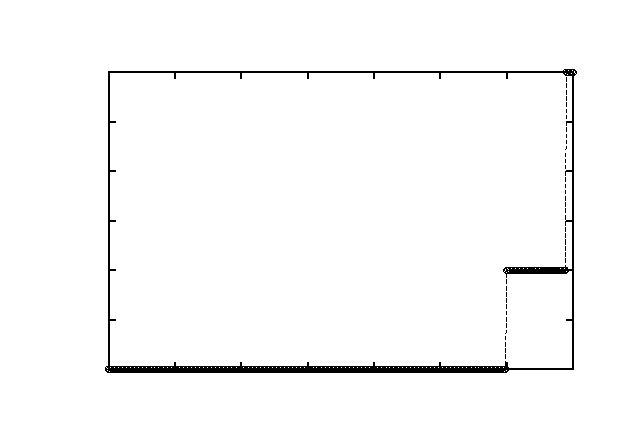
\includegraphics{4-1}}%
    \gplfronttext
  \end{picture}%
\endgroup

	\caption{}
	\label{graph:4-1}
	\end{subfigure}
%
	\hspace{4.0 cm}
%
	\begin{subfigure}[!htp]{0.5\textwidth}
	% GNUPLOT: LaTeX picture with Postscript
\begingroup
  \fontfamily{phv}%
  \selectfont
\definecolor{t}{rgb}{0.5,0.5,0.5}
  \makeatletter
  \providecommand\color[2][]{%
    \GenericError{(gnuplot) \space\space\space\@spaces}{%
      Package color not loaded in conjunction with
      terminal option `colourtext'%
    }{See the gnuplot documentation for explanation.%
    }{Either use 'blacktext' in gnuplot or load the package
      color.sty in LaTeX.}%
    \renewcommand\color[2][]{}%
  }%
  \providecommand\includegraphics[2][]{%
    \GenericError{(gnuplot) \space\space\space\@spaces}{%
      Package graphicx or graphics not loaded%
    }{See the gnuplot documentation for explanation.%
    }{The gnuplot epslatex terminal needs graphicx.sty or graphics.sty.}%
    \renewcommand\includegraphics[2][]{}%
  }%
  \providecommand\rotatebox[2]{#2}%
  \@ifundefined{ifGPcolor}{%
    \newif\ifGPcolor
    \GPcolortrue
  }{}%
  \@ifundefined{ifGPblacktext}{%
    \newif\ifGPblacktext
    \GPblacktextfalse
  }{}%
  % define a \g@addto@macro without @ in the name:
  \let\gplgaddtomacro\g@addto@macro
  % define empty templates for all commands taking text:
  \gdef\gplbacktext{}%
  \gdef\gplfronttext{}%
  \makeatother
  \ifGPblacktext
    % no textcolor at all
    \def\colorrgb#1{}%
    \def\colorgray#1{}%
  \else
    % gray or color?
    \ifGPcolor
      \def\colorrgb#1{\color[rgb]{#1}}%
      \def\colorgray#1{\color[gray]{#1}}%
      \expandafter\def\csname LTw\endcsname{\color{white}}%
      \expandafter\def\csname LTb\endcsname{\color{black}}%
      \expandafter\def\csname LTa\endcsname{\color{black}}%
      \expandafter\def\csname LT0\endcsname{\color[rgb]{1,0,0}}%
      \expandafter\def\csname LT1\endcsname{\color[rgb]{0,1,0}}%
      \expandafter\def\csname LT2\endcsname{\color[rgb]{0,0,1}}%
      \expandafter\def\csname LT3\endcsname{\color[rgb]{1,0,1}}%
      \expandafter\def\csname LT4\endcsname{\color[rgb]{0,1,1}}%
      \expandafter\def\csname LT5\endcsname{\color[rgb]{1,1,0}}%
      \expandafter\def\csname LT6\endcsname{\color[rgb]{0,0,0}}%
      \expandafter\def\csname LT7\endcsname{\color[rgb]{1,0.3,0}}%
      \expandafter\def\csname LT8\endcsname{\color[rgb]{0.5,0.5,0.5}}%
    \else
      % gray
      \def\colorrgb#1{\color{black}}%
      \def\colorgray#1{\color[gray]{#1}}%
      \expandafter\def\csname LTw\endcsname{\color{white}}%
      \expandafter\def\csname LTb\endcsname{\color{black}}%
      \expandafter\def\csname LTa\endcsname{\color{black}}%
      \expandafter\def\csname LT0\endcsname{\color{black}}%
      \expandafter\def\csname LT1\endcsname{\color{black}}%
      \expandafter\def\csname LT2\endcsname{\color{black}}%
      \expandafter\def\csname LT3\endcsname{\color{black}}%
      \expandafter\def\csname LT4\endcsname{\color{black}}%
      \expandafter\def\csname LT5\endcsname{\color{black}}%
      \expandafter\def\csname LT6\endcsname{\color{black}}%
      \expandafter\def\csname LT7\endcsname{\color{black}}%
      \expandafter\def\csname LT8\endcsname{\color{black}}%
    \fi
  \fi
  \setlength{\unitlength}{0.0500bp}%
  \begin{picture}(5668.00,3968.00)%
    \gplgaddtomacro\gplbacktext{%
      \csname LTb\endcsname%
      \put(774,576){\makebox(0,0)[r]{\strut{} 0}}%
      \put(774,861){\makebox(0,0)[r]{\strut{} 10}}%
      \put(774,1146){\makebox(0,0)[r]{\strut{} 20}}%
      \put(774,1431){\makebox(0,0)[r]{\strut{} 30}}%
      \put(774,1716){\makebox(0,0)[r]{\strut{} 40}}%
      \put(774,2002){\makebox(0,0)[r]{\strut{} 50}}%
      \put(774,2287){\makebox(0,0)[r]{\strut{} 60}}%
      \put(774,2572){\makebox(0,0)[r]{\strut{} 70}}%
      \put(774,2857){\makebox(0,0)[r]{\strut{} 80}}%
      \put(774,3142){\makebox(0,0)[r]{\strut{} 90}}%
      \put(774,3427){\makebox(0,0)[r]{\strut{} 100}}%
      \put(882,396){\makebox(0,0){\strut{} 3.5}}%
      \put(1774,396){\makebox(0,0){\strut{} 3.6}}%
      \put(2666,396){\makebox(0,0){\strut{} 3.7}}%
      \put(3559,396){\makebox(0,0){\strut{} 3.8}}%
      \put(4451,396){\makebox(0,0){\strut{} 3.9}}%
      \put(5343,396){\makebox(0,0){\strut{} 4}}%
      \put(144,2001){\makebox(0,0){\strut{}$k$}}%
      \put(3112,126){\makebox(0,0){\strut{}$\lambda$}}%
      \put(3112,3697){\makebox(0,0){\strut{}k vs. $\lambda$ : altos períodos}}%
    }%
    \gplgaddtomacro\gplfronttext{%
    }%
    \gplbacktext
    \put(0,0){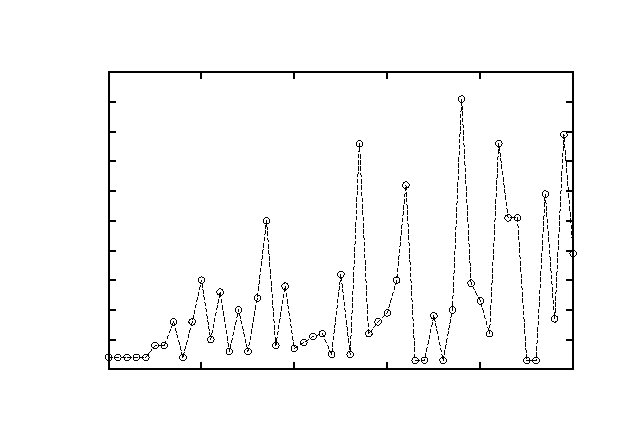
\includegraphics{4-2}}%
    \gplfronttext
  \end{picture}%
\endgroup

	\caption{}
	\label{graph:4-2}
	\end{subfigure}
	\caption{Relações entre $\lambda$, $k$ e $f_k$}
\end{figure}
\FloatBarrier

\section*{Questão 5}
\paragraph{}Consideramos a função:
\begin{equation}
	T(x,t) = T_i + q \left[ 2\sqrt{\frac{\alpha t}{\pi}} e^{-\frac{x^2}{4 \alpha t}} - x \cdot \mbox{erfc}(\frac{x}{2 \sqrt{\alpha t}})\right] 
	\label{eq:T(x,t)}
\end{equation}

\paragraph{}Que determina a temperatura em um ponto $x$ em um instante $t$ de uma barra semi-infinita de temperatura inicial $T_i$ sobre a condição de contorno de um fluxo de calor constante $q$ na origem. Queremos achar quanto tempo um ponto da posição $x_0$ demora para atingir uma temperatura $T_f$ dados $\alpha, T_i$ e $q$ conhecidos. Queremos resolver então o problema:
\begin{displaymath}
	 T(x_0, t) = T_f 
\end{displaymath}
\paragraph{}Ou equivalentemente:
\begin{equation}
	 f(t) = T(x_0, t) - T_f = 0 
	 \label{eq:f(t)}
\end{equation}
\paragraph{}O problema equivale a achar a raiz $t^*$ de $f(t)$ como definido acima. Para isso usamos o método de Newton-Raphson e o processo iterativo é:
\begin{equation}
	t^{(n+1)} = g(t^{(n)}) = t^{(n)} - \frac{f(t^{(n)})}{f'(t^{(n)})}
	\label{eq:newton-raphson}
\end{equation}
\paragraph{}E a raiz $t^*$ de $f(t)$ será também ponto fixo do processo $g(t^{(n)})$.A derivada de f(t) será dada por:
\begin{displaymath}
	f'(t) = \frac{d}{dt} \left( T(x_0, t) - T_f \right) = \frac{\partial}{\partial t} T(x_0, t)
\end{displaymath}

\paragraph{}A derivada parcial de $T(x_0, t)$ será calculada pelo método de \emph{diferenças finitas} de segunda ordem como segue:
\begin{displaymath}
	\frac{\partial}{\partial t} T(x_0, t) \approx \frac{T(x_0, t + \Delta t) - T(x_0, t - \Delta t) }{2 \Delta t}
\end{displaymath}
\paragraph{}Com $\Delta t$ suficientemente pequeno. A função 'erfc(x)' é conhecida como função erro complementar e será aproximada por:
\begin{equation}
	erfc(x) = \frac{1}{(1 + a_1 x + a_2 x^2 + a_3 x^3 + \ldots + a_6 x^6)^{16}}
\end{equation}
\paragraph{}Com os $a_n$'s dados pela aproximação de Abramowitz e Stegun. Dado um chute inicial $t^0$ suficientemente próximo o processo \ref{eq:newton-raphson} é aplicada até que se tenha a precisão desejada.

\section*{Questão 6}
\paragraph{}O método apresentado na seção anterior é implementado para os valores: $T_i = 10$,	 $q = \alpha = x_0 = 1$ e $T_f = 50$.
\paragraph{}Precisamos de um chute inicial para o algoritmo, visando isso vamos estimar a solução por algumas aproximações. Sabe-se que as funções $e^{-\frac{k}{t}}$ e erfc$(\frac{k}{t})$ com $k > 0$ tendem a 1 quando $t$ tende a infinito como pode-se ver no gráfico \ref{graph:exp-erfc}.
\FloatBarrier
\begin{figure}[!htp]
\centering
	% GNUPLOT: LaTeX picture with Postscript
\begingroup
  \fontfamily{phv}%
  \selectfont
\definecolor{t}{rgb}{0.5,0.5,0.5}
  \makeatletter
  \providecommand\color[2][]{%
    \GenericError{(gnuplot) \space\space\space\@spaces}{%
      Package color not loaded in conjunction with
      terminal option `colourtext'%
    }{See the gnuplot documentation for explanation.%
    }{Either use 'blacktext' in gnuplot or load the package
      color.sty in LaTeX.}%
    \renewcommand\color[2][]{}%
  }%
  \providecommand\includegraphics[2][]{%
    \GenericError{(gnuplot) \space\space\space\@spaces}{%
      Package graphicx or graphics not loaded%
    }{See the gnuplot documentation for explanation.%
    }{The gnuplot epslatex terminal needs graphicx.sty or graphics.sty.}%
    \renewcommand\includegraphics[2][]{}%
  }%
  \providecommand\rotatebox[2]{#2}%
  \@ifundefined{ifGPcolor}{%
    \newif\ifGPcolor
    \GPcolortrue
  }{}%
  \@ifundefined{ifGPblacktext}{%
    \newif\ifGPblacktext
    \GPblacktextfalse
  }{}%
  % define a \g@addto@macro without @ in the name:
  \let\gplgaddtomacro\g@addto@macro
  % define empty templates for all commands taking text:
  \gdef\gplbacktext{}%
  \gdef\gplfronttext{}%
  \makeatother
  \ifGPblacktext
    % no textcolor at all
    \def\colorrgb#1{}%
    \def\colorgray#1{}%
  \else
    % gray or color?
    \ifGPcolor
      \def\colorrgb#1{\color[rgb]{#1}}%
      \def\colorgray#1{\color[gray]{#1}}%
      \expandafter\def\csname LTw\endcsname{\color{white}}%
      \expandafter\def\csname LTb\endcsname{\color{black}}%
      \expandafter\def\csname LTa\endcsname{\color{black}}%
      \expandafter\def\csname LT0\endcsname{\color[rgb]{1,0,0}}%
      \expandafter\def\csname LT1\endcsname{\color[rgb]{0,1,0}}%
      \expandafter\def\csname LT2\endcsname{\color[rgb]{0,0,1}}%
      \expandafter\def\csname LT3\endcsname{\color[rgb]{1,0,1}}%
      \expandafter\def\csname LT4\endcsname{\color[rgb]{0,1,1}}%
      \expandafter\def\csname LT5\endcsname{\color[rgb]{1,1,0}}%
      \expandafter\def\csname LT6\endcsname{\color[rgb]{0,0,0}}%
      \expandafter\def\csname LT7\endcsname{\color[rgb]{1,0.3,0}}%
      \expandafter\def\csname LT8\endcsname{\color[rgb]{0.5,0.5,0.5}}%
    \else
      % gray
      \def\colorrgb#1{\color{black}}%
      \def\colorgray#1{\color[gray]{#1}}%
      \expandafter\def\csname LTw\endcsname{\color{white}}%
      \expandafter\def\csname LTb\endcsname{\color{black}}%
      \expandafter\def\csname LTa\endcsname{\color{black}}%
      \expandafter\def\csname LT0\endcsname{\color{black}}%
      \expandafter\def\csname LT1\endcsname{\color{black}}%
      \expandafter\def\csname LT2\endcsname{\color{black}}%
      \expandafter\def\csname LT3\endcsname{\color{black}}%
      \expandafter\def\csname LT4\endcsname{\color{black}}%
      \expandafter\def\csname LT5\endcsname{\color{black}}%
      \expandafter\def\csname LT6\endcsname{\color{black}}%
      \expandafter\def\csname LT7\endcsname{\color{black}}%
      \expandafter\def\csname LT8\endcsname{\color{black}}%
    \fi
  \fi
  \setlength{\unitlength}{0.0500bp}%
  \begin{picture}(5668.00,3968.00)%
    \gplgaddtomacro\gplbacktext{%
      \csname LTb\endcsname%
      \put(594,576){\makebox(0,0)[r]{\strut{} 0.1}}%
      \put(594,929){\makebox(0,0)[r]{\strut{} 0.2}}%
      \put(594,1282){\makebox(0,0)[r]{\strut{} 0.3}}%
      \put(594,1634){\makebox(0,0)[r]{\strut{} 0.4}}%
      \put(594,1987){\makebox(0,0)[r]{\strut{} 0.5}}%
      \put(594,2340){\makebox(0,0)[r]{\strut{} 0.6}}%
      \put(594,2693){\makebox(0,0)[r]{\strut{} 0.7}}%
      \put(594,3045){\makebox(0,0)[r]{\strut{} 0.8}}%
      \put(594,3398){\makebox(0,0)[r]{\strut{} 0.9}}%
      \put(594,3751){\makebox(0,0)[r]{\strut{} 1}}%
      \put(702,396){\makebox(0,0){\strut{} 0}}%
      \put(1630,396){\makebox(0,0){\strut{} 20}}%
      \put(2558,396){\makebox(0,0){\strut{} 40}}%
      \put(3487,396){\makebox(0,0){\strut{} 60}}%
      \put(4415,396){\makebox(0,0){\strut{} 80}}%
      \put(5343,396){\makebox(0,0){\strut{} 100}}%
      \put(3022,126){\makebox(0,0){\strut{}t}}%
    }%
    \gplgaddtomacro\gplfronttext{%
      \csname LTb\endcsname%
      \put(4524,3598){\makebox(0,0)[r]{\strut{}erfc$(k/t)$}}%
      \csname LTb\endcsname%
      \put(4524,3418){\makebox(0,0)[r]{\strut{}\hspace{1 cm}$e^{-k/t}$}}%
    }%
    \gplbacktext
    \put(0,0){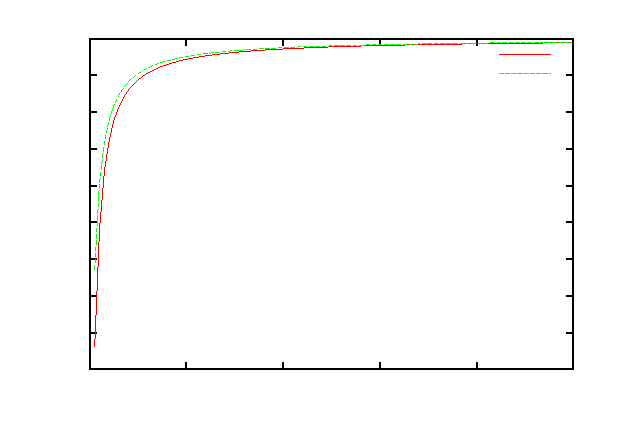
\includegraphics{6-1}}%
    \gplfronttext
  \end{picture}%
\endgroup

	\caption{Comportamento das funções no infinito}
	\label{graph:exp-erfc}
\end{figure}  
\FloatBarrier
 Supomos então que t seja muito grande, então nesse caso a fórmula \ref{eq:T(x,t)} simplifica e obtemos:

\begin{displaymath}
		T(x_0,t) = T_i + q \left[ 2\sqrt{\frac{\alpha t}{\pi}} \cdot 1 - x_0 \cdot  1 \right] 
\end{displaymath}
\paragraph{}Para os valores utilizados nesse problema obtemos nosso chute inicial:
\begin{displaymath}
	t_0 = \pi \frac{(40 + 1)^2}{4} \approx 1320.25
\end{displaymath}

\paragraph{} Vamos calcular a função $f(t)$ definida na equação \ref{eq:f(t)} nas proximidades desse $t_0$:
		\begin{displaymath}
		\begin{tabular}{l}
		$f(1330) = 0.159$ \\
		$f(1300) = -0.308$ 
		\end{tabular}
		\end{displaymath}
\paragraph{}Como $f(t)$ é contínua entre 1300 e 1330, temos pelo teorema do valor médio do cálculo que $f(t)$ possui uma raiz $t^*$ nesse intervalo. 

\paragraph{} O valor $t^*$ calculado pelo algoritmo é:

\begin{equation}
	\centering
	\begin{tabular}{|c|}\hline 
		$t^* = 1319.754395$ \\ \hline
	\end{tabular}
\end{equation}
\paragraph{} E a precisão de 6 casas decimais foi obtida em $n = 3$ iterações. O programa é rodado para alguns valores de chutes iniciais e analisa-se o número de iterações necessárias para que se atinja precisão de 6 casas decimais.Os chutes iniciais começam em 1000 e vão até 15000 com saltos de 100. Os resultados são mostrados no gráfico a seguir. O eixo y é limitado pois processos que não convergem tem $n =\infty$ e esses casos não são interessantes. Os processos que convergem nesse intervalo precisaram de no máximo 8 iterações para convergir. Em nossas simulações limitamos o número de iterações a 1000. Talvez para algum chute inicial sejam necessárias mais iterações mas como os casos que convergiram precisaram de no máximo 8, é difícil acreditar que existam processos convergentes para esse caso em estudo que demorem mais de 1000 iterações. Interpretamos portanto que em 1000 iterações os chutes iniciais que ainda não convergiram é porque divergem independentemente do número de iterações feitas.
\FloatBarrier
\begin{figure}[!htp]
\centering
	% GNUPLOT: LaTeX picture with Postscript
\begingroup
  \fontfamily{phv}%
  \selectfont
\definecolor{t}{rgb}{0.5,0.5,0.5}
  \makeatletter
  \providecommand\color[2][]{%
    \GenericError{(gnuplot) \space\space\space\@spaces}{%
      Package color not loaded in conjunction with
      terminal option `colourtext'%
    }{See the gnuplot documentation for explanation.%
    }{Either use 'blacktext' in gnuplot or load the package
      color.sty in LaTeX.}%
    \renewcommand\color[2][]{}%
  }%
  \providecommand\includegraphics[2][]{%
    \GenericError{(gnuplot) \space\space\space\@spaces}{%
      Package graphicx or graphics not loaded%
    }{See the gnuplot documentation for explanation.%
    }{The gnuplot epslatex terminal needs graphicx.sty or graphics.sty.}%
    \renewcommand\includegraphics[2][]{}%
  }%
  \providecommand\rotatebox[2]{#2}%
  \@ifundefined{ifGPcolor}{%
    \newif\ifGPcolor
    \GPcolortrue
  }{}%
  \@ifundefined{ifGPblacktext}{%
    \newif\ifGPblacktext
    \GPblacktextfalse
  }{}%
  % define a \g@addto@macro without @ in the name:
  \let\gplgaddtomacro\g@addto@macro
  % define empty templates for all commands taking text:
  \gdef\gplbacktext{}%
  \gdef\gplfronttext{}%
  \makeatother
  \ifGPblacktext
    % no textcolor at all
    \def\colorrgb#1{}%
    \def\colorgray#1{}%
  \else
    % gray or color?
    \ifGPcolor
      \def\colorrgb#1{\color[rgb]{#1}}%
      \def\colorgray#1{\color[gray]{#1}}%
      \expandafter\def\csname LTw\endcsname{\color{white}}%
      \expandafter\def\csname LTb\endcsname{\color{black}}%
      \expandafter\def\csname LTa\endcsname{\color{black}}%
      \expandafter\def\csname LT0\endcsname{\color[rgb]{1,0,0}}%
      \expandafter\def\csname LT1\endcsname{\color[rgb]{0,1,0}}%
      \expandafter\def\csname LT2\endcsname{\color[rgb]{0,0,1}}%
      \expandafter\def\csname LT3\endcsname{\color[rgb]{1,0,1}}%
      \expandafter\def\csname LT4\endcsname{\color[rgb]{0,1,1}}%
      \expandafter\def\csname LT5\endcsname{\color[rgb]{1,1,0}}%
      \expandafter\def\csname LT6\endcsname{\color[rgb]{0,0,0}}%
      \expandafter\def\csname LT7\endcsname{\color[rgb]{1,0.3,0}}%
      \expandafter\def\csname LT8\endcsname{\color[rgb]{0.5,0.5,0.5}}%
    \else
      % gray
      \def\colorrgb#1{\color{black}}%
      \def\colorgray#1{\color[gray]{#1}}%
      \expandafter\def\csname LTw\endcsname{\color{white}}%
      \expandafter\def\csname LTb\endcsname{\color{black}}%
      \expandafter\def\csname LTa\endcsname{\color{black}}%
      \expandafter\def\csname LT0\endcsname{\color{black}}%
      \expandafter\def\csname LT1\endcsname{\color{black}}%
      \expandafter\def\csname LT2\endcsname{\color{black}}%
      \expandafter\def\csname LT3\endcsname{\color{black}}%
      \expandafter\def\csname LT4\endcsname{\color{black}}%
      \expandafter\def\csname LT5\endcsname{\color{black}}%
      \expandafter\def\csname LT6\endcsname{\color{black}}%
      \expandafter\def\csname LT7\endcsname{\color{black}}%
      \expandafter\def\csname LT8\endcsname{\color{black}}%
    \fi
  \fi
  \setlength{\unitlength}{0.0500bp}%
  \begin{picture}(5668.00,3968.00)%
    \gplgaddtomacro\gplbacktext{%
      \csname LTb\endcsname%
      \put(666,576){\makebox(0,0)[r]{\strut{} 0}}%
      \put(666,1211){\makebox(0,0)[r]{\strut{} 2}}%
      \put(666,1846){\makebox(0,0)[r]{\strut{} 4}}%
      \put(666,2481){\makebox(0,0)[r]{\strut{} 6}}%
      \put(666,3116){\makebox(0,0)[r]{\strut{} 8}}%
      \put(666,3751){\makebox(0,0)[r]{\strut{} 10}}%
      \put(1100,396){\makebox(0,0){\strut{} 2000}}%
      \put(1753,396){\makebox(0,0){\strut{} 4000}}%
      \put(2406,396){\makebox(0,0){\strut{} 6000}}%
      \put(3059,396){\makebox(0,0){\strut{} 8000}}%
      \put(3711,396){\makebox(0,0){\strut{} 10000}}%
      \put(4364,396){\makebox(0,0){\strut{} 12000}}%
      \put(5017,396){\makebox(0,0){\strut{} 14000}}%
      \put(144,2163){\makebox(0,0){\strut{}n}}%
      \put(3058,126){\makebox(0,0){\strut{}$t_0$}}%
    }%
    \gplgaddtomacro\gplfronttext{%
    }%
    \gplbacktext
    \put(0,0){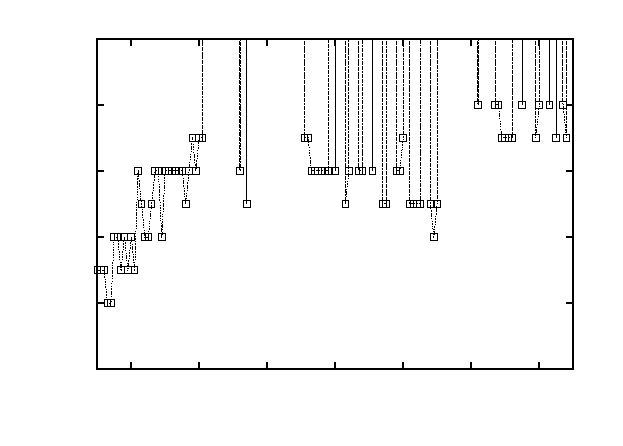
\includegraphics{6-2}}%
    \gplfronttext
  \end{picture}%
\endgroup

	\caption{Número de iterações necessárias para convergência}
	\label{graph:6-2}
\end{figure}  
\FloatBarrier
	\begin{table}[!htp]
		\centering
		\begin{tabular}{|c|c|} \hline
			chute inicial & iterações necessárias \\ \hline
			$t_{0_1} = 2 t_0 = 2640$ & 6 \\ \hline
			$t_{0_2} = 3 t_0 = 3960$ & 6 \\ \hline
			$t_{0_3} = 4 t_0 = 5280$ & $\infty$ \\ \hline
			$t_{0_4} = 5 t_0 = 6600$ & $\infty$  \\ \hline
			$t_{0_5} = 10 t_0 = 13200$ & 7 \\ \hline		
		\end{tabular}
		\caption{Alguns valores particulares de $n(t_{0_k})$}
		\label{table:t-n}		
	\end{table}
\paragraph{}A tabela \ref{table:t-n} mostra o número de iterações necessárias para convergência para alguns valores particulares do chute inicial. Vemos pela tabela e pelo gráfico que não há uma relação óbvia entre o número de iterações necessárias e o chute inicial. Podemos dizer apenas que um chute inicial $t_0$ próximo de $t^*$ tem mais chances de convergir e mais rapidamente.

\section*{Questão 7}
\paragraph{}O método da bisseção é implementado para o mesmo problema. Precisamos para isso de um intervalo no qual procurar a solução. Baseado em nosso chute inicial $t_0 = 1320$ calculamos o valor de $f(t)$ definido na equação \ref{eq:f(t)} em pontos próximos de $t_0$. A tabela \ref{table:7-1} apresenta alguns valores com $t$'s espaçados de 1.
\begin{table}[!htp]
	\centering
	\begin{tabular}{|c|c|}\hline
		$t$	&	f(t) \\ \hline
		1317 & 	 -0.042789 \\ \hline
		1318 	& -0.027248\\ \hline
		1319 	& -0.011715\\ \hline
		$t_0$ = 1320.00 	& 0.003811\\ \hline
		1321 	& 0.019337\\ \hline
		1322 	& 0.034855\\ \hline
		1323 	& 0.050365\\ \hline
	\end{tabular}
	\caption{$f(t)$ em torno de $f(t_0)$}
	\label{table:7-1}
\end{table} 

\paragraph{}Queremos um intervalo centrado em $t_0$ e escolhemos portanto (1319, 1321) como intervalo inicial. Como observa-se uma troca de sinal de $f(t)$ então devemos ter uma raiz nesse intervalo pois f é contínua. Usando esse intervalo o número de iterações necessárias para termos 6 dígitos de precisão é:
	\begin{table}[!htp]
	\centering
		\begin{tabular}{|c|}\hline
			$n = 7$ \\ \hline
		\end{tabular}
	\end{table}

\paragraph{}Esse resultado poderia ser previsto sabendo-se que num intervalo $(a,b)$ o número de iterações necessárias para um erro $\epsilon$ é:
\begin{displaymath}
	n > \log _2 \frac{b - a}{\epsilon} - 1
\end{displaymath}
\paragraph{}Aplicando os valores, obtemos:
\begin{displaymath}
	n > \log _2 \frac{1321 - 1319}{0.01} - 1 = \frac{\log _{10} \frac{2}{0.01}}{\log _{10} 2} - 1 \approx 6.64
\end{displaymath}

\paragraph{}O erro $\epsilon = 0.01$ foi usado pois sabe-se que o valor calculado é da ordem de 1000 e portanto uma precisão de 6 dígitos ocorrerá na segunda casa decimal. Vê-se que o método da bisseção precisou de mais que o dobro de iterações do método de Newton-Raphson para atingir a mesma precisão.

\section*{Questão 8}
\paragraph{} Fixamos agora os mesmos valores de $T_i, T_f, q, \alpha$ e $t_0$ usados na \textbf{questão 6} e fazemos variar o ponto $x_0$ no qual observamos a temperatura. O gráfico \ref{graph:8-1} ilustra o resultado.
\FloatBarrier
\begin{figure}[!htp]
	% GNUPLOT: LaTeX picture with Postscript
\begingroup
  \fontfamily{phv}%
  \selectfont
\definecolor{t}{rgb}{0.5,0.5,0.5}
  \makeatletter
  \providecommand\color[2][]{%
    \GenericError{(gnuplot) \space\space\space\@spaces}{%
      Package color not loaded in conjunction with
      terminal option `colourtext'%
    }{See the gnuplot documentation for explanation.%
    }{Either use 'blacktext' in gnuplot or load the package
      color.sty in LaTeX.}%
    \renewcommand\color[2][]{}%
  }%
  \providecommand\includegraphics[2][]{%
    \GenericError{(gnuplot) \space\space\space\@spaces}{%
      Package graphicx or graphics not loaded%
    }{See the gnuplot documentation for explanation.%
    }{The gnuplot epslatex terminal needs graphicx.sty or graphics.sty.}%
    \renewcommand\includegraphics[2][]{}%
  }%
  \providecommand\rotatebox[2]{#2}%
  \@ifundefined{ifGPcolor}{%
    \newif\ifGPcolor
    \GPcolortrue
  }{}%
  \@ifundefined{ifGPblacktext}{%
    \newif\ifGPblacktext
    \GPblacktextfalse
  }{}%
  % define a \g@addto@macro without @ in the name:
  \let\gplgaddtomacro\g@addto@macro
  % define empty templates for all commands taking text:
  \gdef\gplbacktext{}%
  \gdef\gplfronttext{}%
  \makeatother
  \ifGPblacktext
    % no textcolor at all
    \def\colorrgb#1{}%
    \def\colorgray#1{}%
  \else
    % gray or color?
    \ifGPcolor
      \def\colorrgb#1{\color[rgb]{#1}}%
      \def\colorgray#1{\color[gray]{#1}}%
      \expandafter\def\csname LTw\endcsname{\color{white}}%
      \expandafter\def\csname LTb\endcsname{\color{black}}%
      \expandafter\def\csname LTa\endcsname{\color{black}}%
      \expandafter\def\csname LT0\endcsname{\color[rgb]{1,0,0}}%
      \expandafter\def\csname LT1\endcsname{\color[rgb]{0,1,0}}%
      \expandafter\def\csname LT2\endcsname{\color[rgb]{0,0,1}}%
      \expandafter\def\csname LT3\endcsname{\color[rgb]{1,0,1}}%
      \expandafter\def\csname LT4\endcsname{\color[rgb]{0,1,1}}%
      \expandafter\def\csname LT5\endcsname{\color[rgb]{1,1,0}}%
      \expandafter\def\csname LT6\endcsname{\color[rgb]{0,0,0}}%
      \expandafter\def\csname LT7\endcsname{\color[rgb]{1,0.3,0}}%
      \expandafter\def\csname LT8\endcsname{\color[rgb]{0.5,0.5,0.5}}%
    \else
      % gray
      \def\colorrgb#1{\color{black}}%
      \def\colorgray#1{\color[gray]{#1}}%
      \expandafter\def\csname LTw\endcsname{\color{white}}%
      \expandafter\def\csname LTb\endcsname{\color{black}}%
      \expandafter\def\csname LTa\endcsname{\color{black}}%
      \expandafter\def\csname LT0\endcsname{\color{black}}%
      \expandafter\def\csname LT1\endcsname{\color{black}}%
      \expandafter\def\csname LT2\endcsname{\color{black}}%
      \expandafter\def\csname LT3\endcsname{\color{black}}%
      \expandafter\def\csname LT4\endcsname{\color{black}}%
      \expandafter\def\csname LT5\endcsname{\color{black}}%
      \expandafter\def\csname LT6\endcsname{\color{black}}%
      \expandafter\def\csname LT7\endcsname{\color{black}}%
      \expandafter\def\csname LT8\endcsname{\color{black}}%
    \fi
  \fi
  \setlength{\unitlength}{0.0500bp}%
  \begin{picture}(5668.00,3968.00)%
    \gplgaddtomacro\gplbacktext{%
      \csname LTb\endcsname%
      \put(882,576){\makebox(0,0)[r]{\strut{} 1300}}%
      \put(882,1105){\makebox(0,0)[r]{\strut{} 1350}}%
      \put(882,1634){\makebox(0,0)[r]{\strut{} 1400}}%
      \put(882,2164){\makebox(0,0)[r]{\strut{} 1450}}%
      \put(882,2693){\makebox(0,0)[r]{\strut{} 1500}}%
      \put(882,3222){\makebox(0,0)[r]{\strut{} 1550}}%
      \put(882,3751){\makebox(0,0)[r]{\strut{} 1600}}%
      \put(990,396){\makebox(0,0){\strut{} 1}}%
      \put(1534,396){\makebox(0,0){\strut{} 1.5}}%
      \put(2078,396){\makebox(0,0){\strut{} 2}}%
      \put(2622,396){\makebox(0,0){\strut{} 2.5}}%
      \put(3167,396){\makebox(0,0){\strut{} 3}}%
      \put(3711,396){\makebox(0,0){\strut{} 3.5}}%
      \put(4255,396){\makebox(0,0){\strut{} 4}}%
      \put(4799,396){\makebox(0,0){\strut{} 4.5}}%
      \put(5343,396){\makebox(0,0){\strut{} 5}}%
      \put(144,2163){\makebox(0,0){\strut{}$t^*$}}%
      \put(3166,126){\makebox(0,0){\strut{}$x_0$}}%
    }%
    \gplgaddtomacro\gplfronttext{%
    }%
    \gplbacktext
    \put(0,0){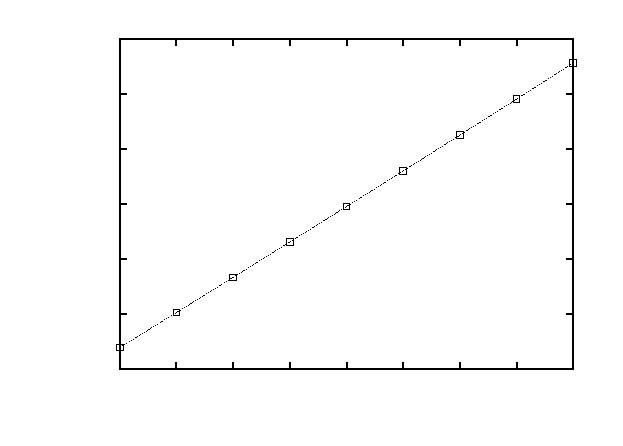
\includegraphics{8-1}}%
    \gplfronttext
  \end{picture}%
\endgroup

	\centering
	\caption{Tempo para $T(x_0, t)$ ir de $T_i$ a $T_f$ em função de $x_0$}
	\label{graph:8-1}
	\end{figure} 
\FloatBarrier
\paragraph{}Os dados podem ser ajustados a uma equação linear e obtemos:
\begin{equation}
	t^*(x_0) =  64.54 x_0  + 1254.55 

\end{equation}

\paragraph{}No gráfico \ref{graph:8-2} vemos a mesma análise mas para alguns valores diferentes de $T_f$. E em seguida vemos as regressões.
\FloatBarrier
\begin{figure}[!htp]
	% GNUPLOT: LaTeX picture with Postscript
\begingroup
  \fontfamily{phv}%
  \selectfont
\definecolor{t}{rgb}{0.5,0.5,0.5}
  \makeatletter
  \providecommand\color[2][]{%
    \GenericError{(gnuplot) \space\space\space\@spaces}{%
      Package color not loaded in conjunction with
      terminal option `colourtext'%
    }{See the gnuplot documentation for explanation.%
    }{Either use 'blacktext' in gnuplot or load the package
      color.sty in LaTeX.}%
    \renewcommand\color[2][]{}%
  }%
  \providecommand\includegraphics[2][]{%
    \GenericError{(gnuplot) \space\space\space\@spaces}{%
      Package graphicx or graphics not loaded%
    }{See the gnuplot documentation for explanation.%
    }{The gnuplot epslatex terminal needs graphicx.sty or graphics.sty.}%
    \renewcommand\includegraphics[2][]{}%
  }%
  \providecommand\rotatebox[2]{#2}%
  \@ifundefined{ifGPcolor}{%
    \newif\ifGPcolor
    \GPcolortrue
  }{}%
  \@ifundefined{ifGPblacktext}{%
    \newif\ifGPblacktext
    \GPblacktextfalse
  }{}%
  % define a \g@addto@macro without @ in the name:
  \let\gplgaddtomacro\g@addto@macro
  % define empty templates for all commands taking text:
  \gdef\gplbacktext{}%
  \gdef\gplfronttext{}%
  \makeatother
  \ifGPblacktext
    % no textcolor at all
    \def\colorrgb#1{}%
    \def\colorgray#1{}%
  \else
    % gray or color?
    \ifGPcolor
      \def\colorrgb#1{\color[rgb]{#1}}%
      \def\colorgray#1{\color[gray]{#1}}%
      \expandafter\def\csname LTw\endcsname{\color{white}}%
      \expandafter\def\csname LTb\endcsname{\color{black}}%
      \expandafter\def\csname LTa\endcsname{\color{black}}%
      \expandafter\def\csname LT0\endcsname{\color[rgb]{1,0,0}}%
      \expandafter\def\csname LT1\endcsname{\color[rgb]{0,1,0}}%
      \expandafter\def\csname LT2\endcsname{\color[rgb]{0,0,1}}%
      \expandafter\def\csname LT3\endcsname{\color[rgb]{1,0,1}}%
      \expandafter\def\csname LT4\endcsname{\color[rgb]{0,1,1}}%
      \expandafter\def\csname LT5\endcsname{\color[rgb]{1,1,0}}%
      \expandafter\def\csname LT6\endcsname{\color[rgb]{0,0,0}}%
      \expandafter\def\csname LT7\endcsname{\color[rgb]{1,0.3,0}}%
      \expandafter\def\csname LT8\endcsname{\color[rgb]{0.5,0.5,0.5}}%
    \else
      % gray
      \def\colorrgb#1{\color{black}}%
      \def\colorgray#1{\color[gray]{#1}}%
      \expandafter\def\csname LTw\endcsname{\color{white}}%
      \expandafter\def\csname LTb\endcsname{\color{black}}%
      \expandafter\def\csname LTa\endcsname{\color{black}}%
      \expandafter\def\csname LT0\endcsname{\color{black}}%
      \expandafter\def\csname LT1\endcsname{\color{black}}%
      \expandafter\def\csname LT2\endcsname{\color{black}}%
      \expandafter\def\csname LT3\endcsname{\color{black}}%
      \expandafter\def\csname LT4\endcsname{\color{black}}%
      \expandafter\def\csname LT5\endcsname{\color{black}}%
      \expandafter\def\csname LT6\endcsname{\color{black}}%
      \expandafter\def\csname LT7\endcsname{\color{black}}%
      \expandafter\def\csname LT8\endcsname{\color{black}}%
    \fi
  \fi
  \setlength{\unitlength}{0.0500bp}%
  \begin{picture}(5668.00,3968.00)%
    \gplgaddtomacro\gplbacktext{%
      \csname LTb\endcsname%
      \put(882,576){\makebox(0,0)[r]{\strut{} 1000}}%
      \put(882,1105){\makebox(0,0)[r]{\strut{} 1500}}%
      \put(882,1634){\makebox(0,0)[r]{\strut{} 2000}}%
      \put(882,2164){\makebox(0,0)[r]{\strut{} 2500}}%
      \put(882,2693){\makebox(0,0)[r]{\strut{} 3000}}%
      \put(882,3222){\makebox(0,0)[r]{\strut{} 3500}}%
      \put(882,3751){\makebox(0,0)[r]{\strut{} 4000}}%
      \put(990,396){\makebox(0,0){\strut{} 0}}%
      \put(1861,396){\makebox(0,0){\strut{} 2}}%
      \put(2731,396){\makebox(0,0){\strut{} 4}}%
      \put(3602,396){\makebox(0,0){\strut{} 6}}%
      \put(4472,396){\makebox(0,0){\strut{} 8}}%
      \put(5343,396){\makebox(0,0){\strut{} 10}}%
      \put(144,2163){\makebox(0,0){\strut{}$t^*$}}%
      \put(3166,126){\makebox(0,0){\strut{}$x_0$}}%
    }%
    \gplgaddtomacro\gplfronttext{%
      \csname LTb\endcsname%
      \put(4524,3598){\makebox(0,0)[r]{\strut{}$T_f = 50$}}%
      \csname LTb\endcsname%
      \put(4524,3418){\makebox(0,0)[r]{\strut{}$T_f = 60$}}%
      \csname LTb\endcsname%
      \put(4524,3238){\makebox(0,0)[r]{\strut{}$T_f = 70$}}%
    }%
    \gplbacktext
    \put(0,0){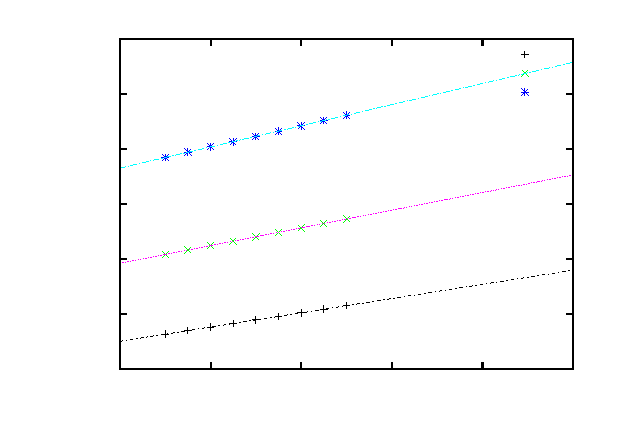
\includegraphics{8-2}}%
    \gplfronttext
  \end{picture}%
\endgroup

	\centering
	\caption{Tempo para $T(x_0, t)$ ir de $T_i$ a $T_f$ em função de $x_0$ para alguns $T_f$'s}
	\label{graph:8-2}
	\end{figure} 
\FloatBarrier
\begin{equation}
\begin{tabular}{l}
	$t^*(x_0)_{T_f = 60} =  80.25 x_0  + 1961.41 
$ \\ 
	$t^*(x_0)_{T_f = 70} =  95.96 x_0  + 2825.34 
$ \\
\end{tabular}
\end{equation}

\paragraph{}Vemos que o coeficiente angular das retas, relacionado à velocidade de propagação da temperatura,  dependem de $T_f$. A intuição nos leva a calcular o quociente ente coeficiente angular $\alpha$ da reta e a diferença de temperatura $\Delta T = T_f - T_i$. Obtemos:
	\begin{table}[!htp]
	\centering
		\begin{tabular}{|l|c|l|}\hline
			$T_f$ & $\alpha$ &  $\frac{\alpha}{\Delta T}$ \\ \hline		
			50 	& 64.54 & 1.6135 \\ \hline
			60 	& 90.25 & 1.6050 \\ \hline				
			70 	& 95.96 & 1.5993 \\ \hline	
		\end{tabular}
	\end{table}
\paragraph{}Baseado nesses 3 casos e tomando $\Delta T$ constante podemos estimar:
\begin{displaymath}
	t^*(x) \approx 1.61 \Delta T x +  k 
\end{displaymath}
\paragraph{}Fazendo uma análise dimensional podemos determinar a unidade dessa constante que achamos:
\begin{displaymath}
\begin{tabular}{ll}
	$[t^*] = s = [1.61]\cdot[\Delta T * x] = [1.61]\cdot [ºC \cdot m]$ & $\Rightarrow [1.61] = \frac{s}{ºC \cdot m} = \frac{1}{ºC \cdot \frac{m}{s}}$
\end{tabular}
\end{displaymath}

\paragraph{}Rescrevemos nossa constante como a divisão pelo sue inverso para obtermos:
\begin{displaymath}
	t^*(x) \approx  \frac{\Delta T x}{0.625 ºC \cdot \frac{m}{s}} +  k 
\end{displaymath}

\paragraph{}E obtemos uma equação da forma $t = \frac{\Delta x}{v}$. Definimos então uma \emph{velocidade de frente de calor} $v_c$ que em nosso caso calculamos como:
\begin{equation}
	v_c = 0.625 ºC \cdot \frac{m}{s}
\end{equation}

\section*{Questão 9}
\paragraph{} Variamos agora $q$ e deixamos o resto constante. O gráfico \ref{graph:9-1} a seguir ilustra o resultado.
\begin{figure}[!htp]
	\centering
	% GNUPLOT: LaTeX picture with Postscript
\begingroup
  \fontfamily{phv}%
  \selectfont
\definecolor{t}{rgb}{0.5,0.5,0.5}
  \makeatletter
  \providecommand\color[2][]{%
    \GenericError{(gnuplot) \space\space\space\@spaces}{%
      Package color not loaded in conjunction with
      terminal option `colourtext'%
    }{See the gnuplot documentation for explanation.%
    }{Either use 'blacktext' in gnuplot or load the package
      color.sty in LaTeX.}%
    \renewcommand\color[2][]{}%
  }%
  \providecommand\includegraphics[2][]{%
    \GenericError{(gnuplot) \space\space\space\@spaces}{%
      Package graphicx or graphics not loaded%
    }{See the gnuplot documentation for explanation.%
    }{The gnuplot epslatex terminal needs graphicx.sty or graphics.sty.}%
    \renewcommand\includegraphics[2][]{}%
  }%
  \providecommand\rotatebox[2]{#2}%
  \@ifundefined{ifGPcolor}{%
    \newif\ifGPcolor
    \GPcolortrue
  }{}%
  \@ifundefined{ifGPblacktext}{%
    \newif\ifGPblacktext
    \GPblacktextfalse
  }{}%
  % define a \g@addto@macro without @ in the name:
  \let\gplgaddtomacro\g@addto@macro
  % define empty templates for all commands taking text:
  \gdef\gplbacktext{}%
  \gdef\gplfronttext{}%
  \makeatother
  \ifGPblacktext
    % no textcolor at all
    \def\colorrgb#1{}%
    \def\colorgray#1{}%
  \else
    % gray or color?
    \ifGPcolor
      \def\colorrgb#1{\color[rgb]{#1}}%
      \def\colorgray#1{\color[gray]{#1}}%
      \expandafter\def\csname LTw\endcsname{\color{white}}%
      \expandafter\def\csname LTb\endcsname{\color{black}}%
      \expandafter\def\csname LTa\endcsname{\color{black}}%
      \expandafter\def\csname LT0\endcsname{\color[rgb]{1,0,0}}%
      \expandafter\def\csname LT1\endcsname{\color[rgb]{0,1,0}}%
      \expandafter\def\csname LT2\endcsname{\color[rgb]{0,0,1}}%
      \expandafter\def\csname LT3\endcsname{\color[rgb]{1,0,1}}%
      \expandafter\def\csname LT4\endcsname{\color[rgb]{0,1,1}}%
      \expandafter\def\csname LT5\endcsname{\color[rgb]{1,1,0}}%
      \expandafter\def\csname LT6\endcsname{\color[rgb]{0,0,0}}%
      \expandafter\def\csname LT7\endcsname{\color[rgb]{1,0.3,0}}%
      \expandafter\def\csname LT8\endcsname{\color[rgb]{0.5,0.5,0.5}}%
    \else
      % gray
      \def\colorrgb#1{\color{black}}%
      \def\colorgray#1{\color[gray]{#1}}%
      \expandafter\def\csname LTw\endcsname{\color{white}}%
      \expandafter\def\csname LTb\endcsname{\color{black}}%
      \expandafter\def\csname LTa\endcsname{\color{black}}%
      \expandafter\def\csname LT0\endcsname{\color{black}}%
      \expandafter\def\csname LT1\endcsname{\color{black}}%
      \expandafter\def\csname LT2\endcsname{\color{black}}%
      \expandafter\def\csname LT3\endcsname{\color{black}}%
      \expandafter\def\csname LT4\endcsname{\color{black}}%
      \expandafter\def\csname LT5\endcsname{\color{black}}%
      \expandafter\def\csname LT6\endcsname{\color{black}}%
      \expandafter\def\csname LT7\endcsname{\color{black}}%
      \expandafter\def\csname LT8\endcsname{\color{black}}%
    \fi
  \fi
  \setlength{\unitlength}{0.0500bp}%
  \begin{picture}(5668.00,3968.00)%
    \gplgaddtomacro\gplbacktext{%
      \csname LTb\endcsname%
      \put(882,576){\makebox(0,0)[r]{\strut{} 0}}%
      \put(882,1030){\makebox(0,0)[r]{\strut{} 200}}%
      \put(882,1483){\makebox(0,0)[r]{\strut{} 400}}%
      \put(882,1937){\makebox(0,0)[r]{\strut{} 600}}%
      \put(882,2390){\makebox(0,0)[r]{\strut{} 800}}%
      \put(882,2844){\makebox(0,0)[r]{\strut{} 1000}}%
      \put(882,3297){\makebox(0,0)[r]{\strut{} 1200}}%
      \put(882,3751){\makebox(0,0)[r]{\strut{} 1400}}%
      \put(990,396){\makebox(0,0){\strut{} 1}}%
      \put(1474,396){\makebox(0,0){\strut{} 2}}%
      \put(1957,396){\makebox(0,0){\strut{} 3}}%
      \put(2441,396){\makebox(0,0){\strut{} 4}}%
      \put(2925,396){\makebox(0,0){\strut{} 5}}%
      \put(3408,396){\makebox(0,0){\strut{} 6}}%
      \put(3892,396){\makebox(0,0){\strut{} 7}}%
      \put(4376,396){\makebox(0,0){\strut{} 8}}%
      \put(4859,396){\makebox(0,0){\strut{} 9}}%
      \put(5343,396){\makebox(0,0){\strut{} 10}}%
      \put(144,2163){\makebox(0,0){\strut{}$t^*$}}%
      \put(3166,126){\makebox(0,0){\strut{}$q$}}%
    }%
    \gplgaddtomacro\gplfronttext{%
      \csname LTb\endcsname%
      \put(4524,3598){\makebox(0,0)[r]{\strut{}$t^*(q)$}}%
    }%
    \gplbacktext
    \put(0,0){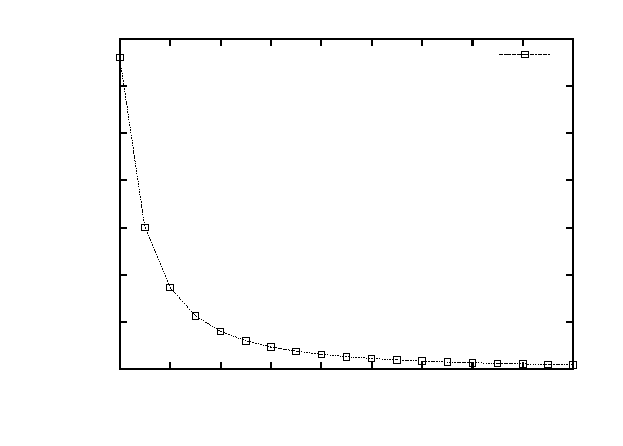
\includegraphics{9-1}}%
    \gplfronttext
  \end{picture}%
\endgroup

	\caption{Tempo para $T(1, t)$ ir de $T_i = 10$ a $T_f = 50$ em função de $q$}
	\label{graph:9-1}
\end{figure} 
\paragraph{}Vemos que com o aumento de $q$ o tempo para a temperatura subir decai de alguma forma exponencial com limite no infinito aparentemente nulo. No próximo experimento variamos $\alpha$ e deixamos o resto constante. Vemos o resultado na figura \ref{graph:9-2}.Notamos que novamente o decaimento é exponencial mas que o limite no infinito é uma constate não nula positiva.
\FloatBarrier
\begin{figure}[!htp]
	\centering
	% GNUPLOT: LaTeX picture with Postscript
\begingroup
  \fontfamily{phv}%
  \selectfont
\definecolor{t}{rgb}{0.5,0.5,0.5}
  \makeatletter
  \providecommand\color[2][]{%
    \GenericError{(gnuplot) \space\space\space\@spaces}{%
      Package color not loaded in conjunction with
      terminal option `colourtext'%
    }{See the gnuplot documentation for explanation.%
    }{Either use 'blacktext' in gnuplot or load the package
      color.sty in LaTeX.}%
    \renewcommand\color[2][]{}%
  }%
  \providecommand\includegraphics[2][]{%
    \GenericError{(gnuplot) \space\space\space\@spaces}{%
      Package graphicx or graphics not loaded%
    }{See the gnuplot documentation for explanation.%
    }{The gnuplot epslatex terminal needs graphicx.sty or graphics.sty.}%
    \renewcommand\includegraphics[2][]{}%
  }%
  \providecommand\rotatebox[2]{#2}%
  \@ifundefined{ifGPcolor}{%
    \newif\ifGPcolor
    \GPcolortrue
  }{}%
  \@ifundefined{ifGPblacktext}{%
    \newif\ifGPblacktext
    \GPblacktextfalse
  }{}%
  % define a \g@addto@macro without @ in the name:
  \let\gplgaddtomacro\g@addto@macro
  % define empty templates for all commands taking text:
  \gdef\gplbacktext{}%
  \gdef\gplfronttext{}%
  \makeatother
  \ifGPblacktext
    % no textcolor at all
    \def\colorrgb#1{}%
    \def\colorgray#1{}%
  \else
    % gray or color?
    \ifGPcolor
      \def\colorrgb#1{\color[rgb]{#1}}%
      \def\colorgray#1{\color[gray]{#1}}%
      \expandafter\def\csname LTw\endcsname{\color{white}}%
      \expandafter\def\csname LTb\endcsname{\color{black}}%
      \expandafter\def\csname LTa\endcsname{\color{black}}%
      \expandafter\def\csname LT0\endcsname{\color[rgb]{1,0,0}}%
      \expandafter\def\csname LT1\endcsname{\color[rgb]{0,1,0}}%
      \expandafter\def\csname LT2\endcsname{\color[rgb]{0,0,1}}%
      \expandafter\def\csname LT3\endcsname{\color[rgb]{1,0,1}}%
      \expandafter\def\csname LT4\endcsname{\color[rgb]{0,1,1}}%
      \expandafter\def\csname LT5\endcsname{\color[rgb]{1,1,0}}%
      \expandafter\def\csname LT6\endcsname{\color[rgb]{0,0,0}}%
      \expandafter\def\csname LT7\endcsname{\color[rgb]{1,0.3,0}}%
      \expandafter\def\csname LT8\endcsname{\color[rgb]{0.5,0.5,0.5}}%
    \else
      % gray
      \def\colorrgb#1{\color{black}}%
      \def\colorgray#1{\color[gray]{#1}}%
      \expandafter\def\csname LTw\endcsname{\color{white}}%
      \expandafter\def\csname LTb\endcsname{\color{black}}%
      \expandafter\def\csname LTa\endcsname{\color{black}}%
      \expandafter\def\csname LT0\endcsname{\color{black}}%
      \expandafter\def\csname LT1\endcsname{\color{black}}%
      \expandafter\def\csname LT2\endcsname{\color{black}}%
      \expandafter\def\csname LT3\endcsname{\color{black}}%
      \expandafter\def\csname LT4\endcsname{\color{black}}%
      \expandafter\def\csname LT5\endcsname{\color{black}}%
      \expandafter\def\csname LT6\endcsname{\color{black}}%
      \expandafter\def\csname LT7\endcsname{\color{black}}%
      \expandafter\def\csname LT8\endcsname{\color{black}}%
    \fi
  \fi
  \setlength{\unitlength}{0.0500bp}%
  \begin{picture}(5668.00,3968.00)%
    \gplgaddtomacro\gplbacktext{%
      \csname LTb\endcsname%
      \put(882,576){\makebox(0,0)[r]{\strut{} 0}}%
      \put(882,1030){\makebox(0,0)[r]{\strut{} 200}}%
      \put(882,1483){\makebox(0,0)[r]{\strut{} 400}}%
      \put(882,1937){\makebox(0,0)[r]{\strut{} 600}}%
      \put(882,2390){\makebox(0,0)[r]{\strut{} 800}}%
      \put(882,2844){\makebox(0,0)[r]{\strut{} 1000}}%
      \put(882,3297){\makebox(0,0)[r]{\strut{} 1200}}%
      \put(882,3751){\makebox(0,0)[r]{\strut{} 1400}}%
      \put(990,396){\makebox(0,0){\strut{} 1}}%
      \put(1474,396){\makebox(0,0){\strut{} 2}}%
      \put(1957,396){\makebox(0,0){\strut{} 3}}%
      \put(2441,396){\makebox(0,0){\strut{} 4}}%
      \put(2925,396){\makebox(0,0){\strut{} 5}}%
      \put(3408,396){\makebox(0,0){\strut{} 6}}%
      \put(3892,396){\makebox(0,0){\strut{} 7}}%
      \put(4376,396){\makebox(0,0){\strut{} 8}}%
      \put(4859,396){\makebox(0,0){\strut{} 9}}%
      \put(5343,396){\makebox(0,0){\strut{} 10}}%
      \put(144,2163){\makebox(0,0){\strut{}$t^*$}}%
      \put(3166,126){\makebox(0,0){\strut{}$\alpha$}}%
    }%
    \gplgaddtomacro\gplfronttext{%
      \csname LTb\endcsname%
      \put(4524,3598){\makebox(0,0)[r]{\strut{}$t^*(\alpha)$}}%
    }%
    \gplbacktext
    \put(0,0){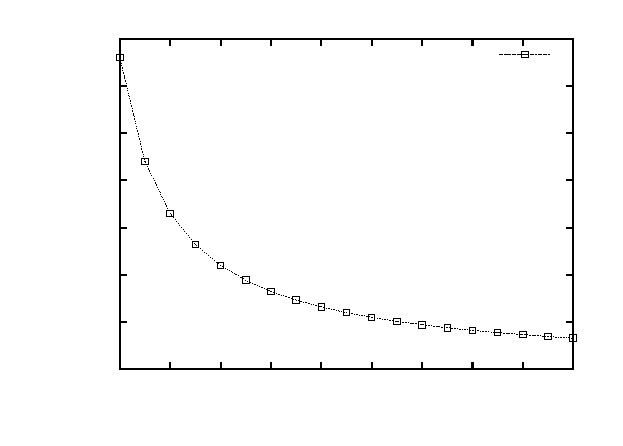
\includegraphics{9-2}}%
    \gplfronttext
  \end{picture}%
\endgroup

	\caption{Tempo para $T(1, t)$ ir de $T_i = 10$ a $T_f = 50$ em função de $\alpha$}
	\label{graph:9-2}
\end{figure} 
\FloatBarrier

\paragraph{} Vemos que ambos os gráficos representam o esperado do senso comum. Se o maçarico for muito forte, ou seja, q for muito alto espera-se que a barra inteira se aqueça rapidamente sendo o tempo de aquecimento zero se q for infinito. Quanto a $\alpha$ vemos que quanto mais facilmente o corpo transporta calor mais uniformemente o corpo se aquece. No caso em que a difusividade térmica for infinita o corpo aquece homogêniamente, o que não quer dizer que o tempo de aquecimento seja 0 mas sim uma constante que depende provavelmente do tamanho da barra, seu calor específico e da intensidade do maçarico. 

\newpage
\section*{Questão 10}
\paragraph{}Analisamos agora o erro das aproximações $t^{(k)}$ em cada iteração $k$ tomando o valor de $t^*$ achado após muitas iterações como correto para cada um dos dois algoritmos utilizados. Espera-se que o erro decaia mais rapidamente no algoritmo de Newton-Raphson que no da bisseção. Plotamos também a curva $\frac{1}{n^2}$ para compararmos as duas convergências com uma convergência quadrática.

\FloatBarrier
\begin{figure}[!htp]
	\centering
	% GNUPLOT: LaTeX picture with Postscript
\begingroup
  \makeatletter
  \providecommand\color[2][]{%
    \GenericError{(gnuplot) \space\space\space\@spaces}{%
      Package color not loaded in conjunction with
      terminal option `colourtext'%
    }{See the gnuplot documentation for explanation.%
    }{Either use 'blacktext' in gnuplot or load the package
      color.sty in LaTeX.}%
    \renewcommand\color[2][]{}%
  }%
  \providecommand\includegraphics[2][]{%
    \GenericError{(gnuplot) \space\space\space\@spaces}{%
      Package graphicx or graphics not loaded%
    }{See the gnuplot documentation for explanation.%
    }{The gnuplot epslatex terminal needs graphicx.sty or graphics.sty.}%
    \renewcommand\includegraphics[2][]{}%
  }%
  \providecommand\rotatebox[2]{#2}%
  \@ifundefined{ifGPcolor}{%
    \newif\ifGPcolor
    \GPcolorfalse
  }{}%
  \@ifundefined{ifGPblacktext}{%
    \newif\ifGPblacktext
    \GPblacktexttrue
  }{}%
  % define a \g@addto@macro without @ in the name:
  \let\gplgaddtomacro\g@addto@macro
  % define empty templates for all commands taking text:
  \gdef\gplbacktext{}%
  \gdef\gplfronttext{}%
  \makeatother
  \ifGPblacktext
    % no textcolor at all
    \def\colorrgb#1{}%
    \def\colorgray#1{}%
  \else
    % gray or color?
    \ifGPcolor
      \def\colorrgb#1{\color[rgb]{#1}}%
      \def\colorgray#1{\color[gray]{#1}}%
      \expandafter\def\csname LTw\endcsname{\color{white}}%
      \expandafter\def\csname LTb\endcsname{\color{black}}%
      \expandafter\def\csname LTa\endcsname{\color{black}}%
      \expandafter\def\csname LT0\endcsname{\color[rgb]{1,0,0}}%
      \expandafter\def\csname LT1\endcsname{\color[rgb]{0,1,0}}%
      \expandafter\def\csname LT2\endcsname{\color[rgb]{0,0,1}}%
      \expandafter\def\csname LT3\endcsname{\color[rgb]{1,0,1}}%
      \expandafter\def\csname LT4\endcsname{\color[rgb]{0,1,1}}%
      \expandafter\def\csname LT5\endcsname{\color[rgb]{1,1,0}}%
      \expandafter\def\csname LT6\endcsname{\color[rgb]{0,0,0}}%
      \expandafter\def\csname LT7\endcsname{\color[rgb]{1,0.3,0}}%
      \expandafter\def\csname LT8\endcsname{\color[rgb]{0.5,0.5,0.5}}%
    \else
      % gray
      \def\colorrgb#1{\color{black}}%
      \def\colorgray#1{\color[gray]{#1}}%
      \expandafter\def\csname LTw\endcsname{\color{white}}%
      \expandafter\def\csname LTb\endcsname{\color{black}}%
      \expandafter\def\csname LTa\endcsname{\color{black}}%
      \expandafter\def\csname LT0\endcsname{\color{black}}%
      \expandafter\def\csname LT1\endcsname{\color{black}}%
      \expandafter\def\csname LT2\endcsname{\color{black}}%
      \expandafter\def\csname LT3\endcsname{\color{black}}%
      \expandafter\def\csname LT4\endcsname{\color{black}}%
      \expandafter\def\csname LT5\endcsname{\color{black}}%
      \expandafter\def\csname LT6\endcsname{\color{black}}%
      \expandafter\def\csname LT7\endcsname{\color{black}}%
      \expandafter\def\csname LT8\endcsname{\color{black}}%
    \fi
  \fi
  \setlength{\unitlength}{0.0500bp}%
  \begin{picture}(5668.00,3968.00)%
    \gplgaddtomacro\gplbacktext{%
      \csname LTb\endcsname%
      \put(946,704){\makebox(0,0)[r]{\strut{} 0}}%
      \put(946,1204){\makebox(0,0)[r]{\strut{} 0.1}}%
      \put(946,1704){\makebox(0,0)[r]{\strut{} 0.2}}%
      \put(946,2204){\makebox(0,0)[r]{\strut{} 0.3}}%
      \put(946,2703){\makebox(0,0)[r]{\strut{} 0.4}}%
      \put(946,3203){\makebox(0,0)[r]{\strut{} 0.5}}%
      \put(946,3703){\makebox(0,0)[r]{\strut{} 0.6}}%
      \put(1078,484){\makebox(0,0){\strut{} 0}}%
      \put(1917,484){\makebox(0,0){\strut{} 2}}%
      \put(2755,484){\makebox(0,0){\strut{} 4}}%
      \put(3594,484){\makebox(0,0){\strut{} 6}}%
      \put(4432,484){\makebox(0,0){\strut{} 8}}%
      \put(5271,484){\makebox(0,0){\strut{} 10}}%
      \put(176,2203){\makebox(0,0){\strut{}$|\frac{t^{(n)} - t^*}{t^*}|$}}%
      \put(3174,154){\makebox(0,0){\strut{}$n$}}%
    }%
    \gplgaddtomacro\gplfronttext{%
      \csname LTb\endcsname%
      \put(4284,3530){\makebox(0,0)[r]{\strut{}Newton-Raphson}}%
      \csname LTb\endcsname%
      \put(4284,3310){\makebox(0,0)[r]{\strut{}Bisseção}}%
      \csname LTb\endcsname%
      \put(4284,3090){\makebox(0,0)[r]{\strut{}$\frac{1}{n^2}$}}%
    }%
    \gplbacktext
    \put(0,0){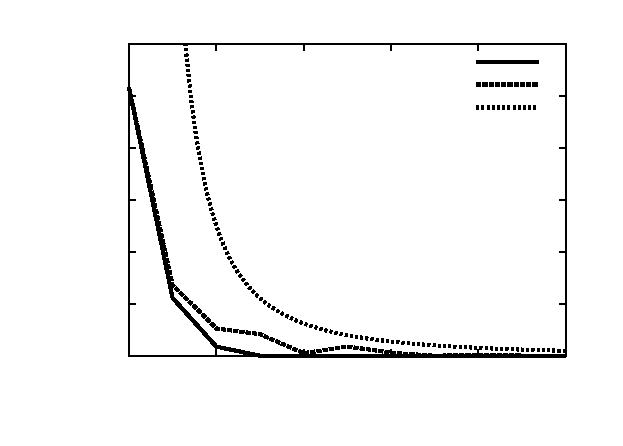
\includegraphics{10-1}}%
    \gplfronttext
  \end{picture}%
\endgroup

	\caption{Erro percentual por n para os dois algoritmos}
	\label{}
\end{figure} 
\FloatBarrier

\paragraph{}Notamos que a curva da bisseção sobe um pouco na 5ª iteração o que pode parecer um erro a princípio. Vamos analisar isso melhor. Digamos que para um certo passo da iteração tenhamos:
\begin{displaymath}
\begin{tabular}{llll}
$w^{(n)} = t^* + \epsilon$ &, $u^{(n)} = t^* - \Delta _1 $ &, $v^{(n)} = t^* + \Delta _2 $ & e $f(u^{(n)}) \cdot f(w^{(n)}) < 0$
\end{tabular}
\end{displaymath}  Nesse caso $v^{(n+1)} = w^{(n)}$ e então:
	\begin{displaymath}
		\begin{tabular}{ll}
			$w^{(n+1)} = \frac{(t^* - \Delta_1 + t^* + \epsilon)}{2} $ & $= t^* + \frac{\epsilon - \Delta_1}{2}$
		\end{tabular}
	\end{displaymath}
	
	\paragraph{}É claro então que é possível que $w^{(n+1)}$ esteja mais longe de $t^*$ do que $w^{(n)}$. Isso deve acontecer sempre que $w^{(n)}$ for quase $t^*$. O comportamento do erro segue portanto o esperado e ambos os algoritmos decaem de forma   mais rápida do que a quadrática. 
\newpage
\section*{Códigos}

\subsection*{Mapa Logístico}

    \begin{enumerate}
        \item \textbf{Impressão do mapa logístico}.
		\hspace{-2.5 cm}
            \begin{lstlisting}
int main(int argc, char* argv[]){

	int n;//indexa a iteracao
	float lambda, x;
	FILE *fp;

	fp = fopen("./data/3-1.dat", "w+");

	for(lambda = 0; lambda <= 4;  lambda += 0.001)
		{
		x = 0.5;//chute inicial
		for(n = 0; n < 200; n++)//descartadas 	
			x = lambda*x*(1 - x);
		for(n = 0; n < 50; n++)//imprimidas
			{
			x = lambda*x*(1 - x);
			fprintf(fp, "%.5f \t %.6f\n", lambda, x);
			}//end for
			
		}//end for

	fclose(fp);
			
	return(0);
	}

            \end{lstlisting}
            \newpage
     \item \textbf{Calculando períodos}
     	\begin{lstlisting}
    int main(int argc, char* argv[]){

	int n, periodo;
	float lambda, x, x_f;\\x_f: x a ser achado
	FILE *fp;

	fp = fopen("./data/4-1.dat", "w+");

	for(lambda = 0; lambda <= 4;  lambda += 0.01)
		{
		x = 0.5;
		for(n = 0; n < 300; n++)//descartados	
				x = lambda*x*(1 - x);
		x_f = x;
		periodo = 0;
		for(n = 0; n < 800; n++)//procurando valor repetido
			{
			x = lambda*x*(1 - x);
			periodo++;	
			if(mod(x_f - x) < 0.01) break;
			//0.01 = margem de erro
			}
		fprintf(fp, "%.3f \t %d\n", lambda, periodo);
		}\end for

	fclose(fp);

	return(0);	
	}
     	\end{lstlisting}
    \end{enumerate}
    
    \newpage
   
   \subsection*{Problema de Temperatura numa Barra}
   \begin{enumerate}
   	\item \textbf{Funções Matemáticas e Variáveis Globais}
     	\begin{lstlisting}
//-----------------
//variaveis globais
//-----------------

float *a;//constantes de Abramowitz e Stegun

const float pi = 3.141592654;
float alpha;
float q;
float Ti;
float Tf;
float x0;
//-----------------
//Funcoes Matematicas
//-----------------
float mod(float x){
//modulo de x
	return((x > 0)? x : -1.0*x);
	}
 
float Erfc(float x){
	//funcao erro complementar de x
	int i;
	float result;

	result = 0;
	for(i = 0; i <=6; i++)
		result += a[i]*pow(x, i);
	/constantes a serem definifas em main()
	result = pow(result, -16);
	return(result);
	}

float T(float x, float t){
//funcao temperatura
	double T_xt;
		T_xt = Ti + q * (2* sqrt(alpha*t/pi) //...
* exp(-1*pow(x, 2)/(4*alpha*t)) - x*Erfc(x/(2*sqrt(alpha*t))));
	return(T_xt);
	}
     	\end{lstlisting} \newpage
\begin{lstlisting}
float f(float t){
//funcao da qual procuramos raizes
	return(T(x0, t) - Tf);
	}

float df(float t){
//derivada de f por diferencas finitas de 2 ordem
	float result, dt;

	dt = 0.0005;
	result = (f(t + dt) - f(t - dt))/(2*dt);
	return(result);
	}

float g(float t_n){
//funcao p o metodo de Newton-Raphson
	float result;

	result = t_n - f(t_n)/df(t_n);
	return(result);
	}

     	\end{lstlisting}   
\newpage
   	\item \textbf{Algoritmo de Newton-Raphson}
     	\begin{lstlisting}
int main(int argc, char* argv[]){
	/*------------------------------------------
	 *------------VARIaVEIS GLOGBAIS------------
	 *------------------------------------------ */
	a =(float *)malloc(7*sizeof(float));
	a[0] = 1.0;
	a[1] = 0.0705230784;
	a[2] = 0.0422820123;
	a[3] = 0.0092705272;
	a[4] = 0.0001520143;
	a[5] = 0.0002765672;
	a[6] = 0.0000430638;

	alpha = 1.0;
	q = 1.0;
	Ti = 10;
	Tf = 50;
	x0 = 1 ;

	/*------------------------------------------
	 *------------VARIaVEIS LOCAIS--------------
	 *------------------------------------------ */
	FILE *f_out;
	float t, t_ant, t_0; 
	//t anterior e t inicial
	int n_iterations;//indexa iteracao
	
	f_out = fopen("./data/6.dat", "w");

	t = t_0;
	for(n_iterations = 0 ; n_iterations <= 100; n_iterations ++)
		{
		t_ant = t;
		//guaradamos t_ant para comparacao de precisao 
		t = g(t);
		if((int)(t*pow(10, 2) - t_ant*pow(10, 2)) == 0) break;
		//precisao de 6 digitos			
		}//end for
	fprintf(f_out, "%.3f \t %d \n", t, n_iterations);

	fclose(f_out);
return(0);}
     	\end{lstlisting}   
\newpage
\item \textbf{Método da Bisseção} 

\begin{lstlisting}   
int main(){
	alpha = 1.0;
	q = 1.0;
	Ti = 10;
	Tf = 50;
	x0 = 1 ;
	/*------------------------------------------
	 *------------VARIaVEIS LOCAIS------------
	 *------------------------------------------ */


	float u, v, w, t_0;
	float a, b;
	int n, k;
	FILE *f_out;

	f_out = fopen("./data/7-1.dat", "w+");

	n = 1600;//limite de iteracoes
	t_0 = 1320;//centro do intervalo

	a = t_0 - 1;
	b = t_0 + 1;
	if(f(a)*f(b) >= 0)
		{
		printf("Metodo da Bissecao nao aplicavel! \n");
		return(0);
		}

	u = a;//limite esquerdo inicial
	v = b;//limite direito inicial
	for(k = 0; k < n; k++)
		{
			w = (u + v)/2.0;
			if(f(w) == 0)	break;
			if(f(u)*f(w) < 0)	v = w;
			else u = w;
			fprintf(f_out, "%f\t %d\n", w, k);
		}

	fclose(f_out);
	return(0);}
\end{lstlisting}   

   \end{enumerate}
   

%@@@@@@@@@@@@@@@@@@@@@@@@@@@@@@@@@@@@@@@@@@@@@@@@@@@@@@@@@@@
%@@@@@@@@@@@@@@       REFERÊNCIAS     @@@@@@@@@@@@@@@@@@@@@@
%@@@@@@@@@@@@@@@@@@@@@@@@@@@@@@@@@@@@@@@@@@@@@@@@@@@@@@@@@@@
\begin{thebibliography}{9}    
	 \bibitem{CN}
   		Oliver, P.J;
  		\emph{Numerical Analysis Lecture Notes} cap. 2 : Numerical Solution of Scalar Equations.
\end{thebibliography}



\end{document}
